%%
%% This is file `thesis.tex',
%% generated with the docstrip utility.
%%
%% The original source files were:
%%
%% nudtpaper.dtx  (with options: `thesis')
%% 
%% This is a generated file.
%% 
%% Copyright (C) 2018 by TomHeaven <hanlin_tan@nudt.edu.cn>
%% 
%% This file may be distributed and/or modified under the
%% conditions of the LaTeX Project Public License, either version 1.3a
%% of this license or (at your option) any later version.
%% The latest version of this license is in:
%% 
%% To produce the documentation run the original source files ending with `.dtx'
%% through LaTeX.
%% 
%% Thanks LiuBenYuan <liubenyuan@gmail.com> for maintainence.
%% Thanks Xue Ruini <xueruini@gmail.com> for the thuthesis class!
%% Thanks sofoot for the original NUDT paper class!
%% 
%1. 规范硕士导言
% \documentclass[master,ttf]{nudtpaper}
%2. 规范博士导言
% \documentclass[doctor,twoside,ttf]{nudtpaper}
%3. 如果使用是Vista
% \documentclass[master,ttf,vista]{nudtpaper}
%4. 建议使用ttf字体
% \documentclass[doctor,twoside,fz]{nudtpaper}
%5. 如果想生成盲评,传递anon即可,仍需修改个人成果部分
% \documentclass[master,otf,anon]{nudtpaper}
%
\documentclass[master,ttf]{nudtpaper}
\usepackage{mynudt}
\usepackage{multirow,array,makecell}

\classification{TP391}
\serialno{231202114}
\confidentiality{公开}
\UDC{681}
\title{面向跨软件生态的兼容性问题\\分析与检测}
\displaytitle{面向跨软件生态的兼容性问题分析与检测}
\author{谢一帆}
\zhdate{\zhtoday}
\entitle{Analysing and Detecting Cross-ecosystem Compatibility Issues}
\enauthor{Yifan Xie}
\endate{\entoday}
\subject{软件工程}
\ensubject{Software Engineering}
\researchfield{智能化软件工程}
\supervisor{刘晓东\quad{}副研究员}
\cosupervisor{李姗姗\quad{}教授}  % 协助指导教师,没有就空着
\ensupervisor{Assoc. Prof. Xiaodong Liu}
\encosupervisor{Prof. Shanshan Li} % 协助指导教师英文,没有就空着
\papertype{工学}
\enpapertype{Engineering}
% 加入makenomenclature命令可用nomencl制作符号列表。

\begin{document}
	\graphicspath{{figures/}}
	% 制作封面,生成目录,插入摘要,插入符号列表 \\
	% 默认符号列表使用denotation.tex,如果要使用nomencl \\
	% 需要注释掉denotation,并取消下面两个命令的注释。 \\
	% cleardoublepage% \\
	% printnomenclature% \\
\maketitle
\frontmatter
\tableofcontents
\listoftables
\listoffigures

\midmatter
\begin{cabstract}
在现代软件开发中,使用第三方包成为了软件复用的重要手段。随着软件领域的不断演进,各类软件生态的通用做法是将越来越多的第三方包发布并维护在一个中央仓库中,以便开发者下载和安装。这种方式极大的提高了软件开发效率,但也给开发者维护第三方包兼容性带来了新的挑战。

目前,随着编程语言的飞速发展,许多语言都建立了自己的软件生态,与此同时,操作系统作为基础软件的代表,也演化出了以各种linux发行版为代表的操作系统生态。
两类生态都将可复用的软件代码打包并发布在公开的第三方包仓库中,并且它们一般都提供了服务于自身生态仓库的包管理工具,帮助用户管理第三方包并处理第三方包的依赖关系,
这些工具通常都经过精心设计来处理仓库内部的第三方包依赖关系,但是不考虑仓库间的第三方包依赖关系。
然而,由于用户往往需要使用来自不同仓库的软件包,可能会出现跨软件生态的兼容性问题(CC问题)。现有研究通常只关注单一软件仓库,无法检测CC问题。为了填补这一空白,本文以Python语言生态和Ubuntu系统生态为代表,将重点关注以下两个研究问题:(1)不同软件仓库中的第三方包发生兼容性问题的根本原因是什么?(2)如何预测、检测和修复CC问题?

基于以上问题和总结,本文深入分析CC问题,并进行了如下探索性工作:
\begin{itemize}
	\item 本文从Ubuntu系统软件仓库,Python软件仓库和Python解释器出发,研究不同仓库间Python软件包的兼容性问题。首先,本文系统性的探讨了Ubuntu包管理工具apt和Python包管理工具pip的依赖解析规则,然后深入分析了系统级Python解释器的包调用规则。基于上述分析,本研究总结了CC问题的触发模式和表现形式,并在Ubuntu生态软件仓库和Python软件仓库间,建立了一个包含1692个CC问题的数据集。
	\item 在上述分析的基础上,本研究设计了一款自动解决 CC 问题的工具 Hera。Hera 首先离线建立一个跨生态兼容性数据库、然后在线预测、检测和修复用户系统环境中的 CC 问题。实验结果显示,Hera在上述CC问题数据集上的检测准确率为 90.5\%,召回率为 93.7\%。我们还从GitHub和Stack Overflow收集并复现了26 个CC问题,Hera成功检测出了所有这些问题并提供了正确的修复建议。
\end{itemize}
\end{cabstract}
\ckeywords{Ubuntu生态; Python生态; 兼容性问题}

\begin{eabstract}
In modern software development, using third-party packages has become an important means of software reuse.
With the continuous evolution of the software field, the common practice across various software ecosystems is to publish and maintain an increasing number of third-party packages in a central repository for developers to download and install.
This approach significantly enhances software development efficiency, but it also introduces new challenges for developers in maintaining compatibility of third-party packages.

At present, with the rapid development of programming languages, many languages have established their own software ecosystems. At the same time, as a representative of foundational software, operating systems have also evolved into various Linux distributions, forming distinct OS ecosystems.
Both types of ecosystems package reusable software code and publish it in public third-party repositories, and they generally provide package management tools that serve their own ecosystem repositories to help users manage third-party packages and handle their dependencies.
These tools are usually designed with great care to handle intra-repository third-party package dependencies but do not consider inter-repository package dependencies.
However, since users often need to use packages from different repositories, cross-ecosystem compatibility issues (CC issues) may arise.
Existing research usually focuses on a single software repository and cannot detect CC issues.
To fill this gap, this paper takes the Python language ecosystem and the Ubuntu system ecosystem as representatives and focuses on the following two research questions: (1) What are the root causes of compatibility issues between third-party packages in different software repositories? (2) How to predict, detect, and resolve CC issues?

Based on the above questions and summary, this paper conducts an in-depth analysis of CC issues and undertakes the following exploratory work:
\begin{itemize}
	\item This paper investigates compatibility issues between Python packages across different repositories, starting from the Ubuntu system software repository, Python software repository, and Python interpreter.
	First, this paper systematically explores the dependency resolution rules of Ubuntu's package manager apt and Python's package manager pip, and then delves into the package invocation rules of the system-level Python interpreter.
	Based on the above analysis, this study summarizes the triggering patterns and manifestations of CC issues and establishes a dataset containing 1,692 CC issues between the Ubuntu ecosystem software repository and the Python software repository.
	\item Based on the above analysis, this study designed an automated tool named Hera to resolve CC issues.
	Hera first establishes an offline cross-ecosystem compatibility database, and then predicts, detects, and resolves CC issues in the user's system environment online.
	Experimental results show that Hera achieves a detection accuracy of 90.5\% and a recall rate of 93.7\% on the aforementioned CC issue dataset.
	We also collected and reproduced 26 CC issues from GitHub and Stack Overflow, and Hera successfully detected all these issues and provided correct repair suggestions.
\end{itemize}


\end{eabstract}
\ekeywords{Ubuntu Ecosystem; Python Ecosystem; Compatibility Issues}


\chapter*{符号使用说明}
% 可以根据需要在chapter后加星星/去掉星星

\begin{denotation}

\item[HPC] 高性能计算 (High Performance Computing)
\item[cluster] 集群
\item[Itanium] 安腾
\item[SMP] 对称多处理
\item[API] 应用程序编程接口
\item[PI]	聚酰亚胺
\item[MPI]	聚酰亚胺模型化合物,N-苯基邻苯酰亚胺
\item[PBI]	聚苯并咪唑
\item[MPBI]	聚苯并咪唑模型化合物,N-苯基苯并咪唑
\item[PY]	聚吡咙
\item[PMDA-BDA]	均苯四酸二酐与联苯四胺合成的聚吡咙薄膜
\item[$\Delta G$]  	活化自由能~(Activation Free Energy)
\item [$\chi$] 传输系数~(Transmission Coefficient)
\item[$E$] 能量
\item[$m$] 质量
\item[$c$] 光速
\item[$P$] 概率
\item[$T$] 时间
\item[$v$] 速度

\end{denotation}

%
%书写正文,可以根据需要增添章节; 正文还包括致谢,参考文献与成果
\mainmatter
\renewcommand\UrlFont{\timesnr}
\makeatletter
\newcounter{blankpages}
\def\cleardoublepage{%
	\clearpage
	\if@twoside
	\ifodd\c@page
	\else
	\hbox{}\newpage\stepcounter{blankpages}%
	\thispagestyle{empty}%
	\if@twocolumn\hbox{}\newpage\fi
	\fi
	\fi
}
\newcommand{\@romannoblank}[1]{%
	\@roman{\numexpr#1-\value{blankpages}\relax}%
}
\makeatother

\chapter{绪论}
在现代软件开发中,使用第三方库成为了软件复用的重要手段之一,第三方库兼容性问题也在软件可靠性领域被视为一个重要的研究点。近年来,随着软件领域的不断演进,各类软件生态蓬勃发展,演化出了成千上万的第三方库,极大的提高了软件开发效率。与此同时,数量如此庞大且依赖关系复杂的第三方库也给用户管理和使用第三方库带来了较大的成本。为了缓解这一问题,各类软件生态提供了包管理工具,帮助用户避免第三方库之间发生兼容性问题。然而,包管理工具往往被设计用于管理自身软件生态的第三方库,却忽视了用户可能会同时使用来自不同软件生态的第三方库,它们之间也可能发生兼容性问题。因此,针对来自不同软件生态的第三方库的兼容性进行分析和检测,对于保障软件依赖可靠性具有关键意义。本章首先阐述了跨软件生态的兼容性问题研究的背景和重要性。然后,介绍了本研究的相关研究工作并总结了现有工作的局限性。接下来,详细描述了本文的研究内容和主要贡献。最后,概述了本文的整体结构。

\section{研究背景及意义}
第三方库(也称为第三方依赖或软件包)是软件开发中重要的可复用资源,可在不依赖其他库的情况下独立安装或删除\upcite{artho2012software}。在现代信息技术飞速发展的背景下,软件项目的规模不断扩展,同时对第三方库的依赖性也逐步增强。已有研究指出,许多项目直接依赖于多个不同的库,且往往因库间依赖关系而间接增加更多依赖\upcite{wang2018dependency}。虽然第三方库极大地提升了项目开发效率,但这种层层叠加的依赖网络可能隐蔽地引入更多的库,增加项目的复杂性和潜在风险\upcite{artho2012software,wang2018dependency,vasilakis2018breakapp,kula2017impact,liang1998dynamic}。
例如,当项目所需的功能(如特定方法)未被加载的第三方库覆盖时,便会出现兼容性问题。当前,开发人员主要依靠经验和技术知识来解决这些问题,这不仅耗费大量时间,还涉及高昂的人力成本。运行时出现的错误报告往往不能有效帮助开发人员定位问题根源。此外,由于第三方库之间存在复杂的相互调用关系,修改一个库可能会影响到其他库的功能,从而增加了问题的解决难度。兼容性问题通常伴随着一些特有的困难,如问题难以重现、编译器的错误报告不够明确、第三方库代码缺失或难于调试等,这些都给开发者管理第三方库带来了额外的挑战。

为了应对这些问题,现代软件开发生态已普遍将大量第三方库打包(第三方包)并维护在中央仓库中,以便开发者能够方便地下载和安装。此外,为了帮助开发者处理第三方包之间复杂的依赖关系并减少兼容性问题,各大软件生态系统均提供了包管理工具,一些著名的软件生态及其包管理工具见图\ref{fig:bac}。在编程语言社区中,Python社区的包管理工具pip管理着近五十万个包,JavaScript的包管理工具npm管理着超过三百万个包\upcite{王莹2023开源软件库生态治理技术研究综述}。在操作系统领域,Ubuntu的包管理工具apt和Fedora的包管理工具dnf也分别管理着大量的deb和rpm包,这些工具不仅支持包的下载和删除,还提供依赖解析等功能,有效地支持开发者管理和使用第三方包。这种集中化的管理模式不仅提高了软件开发的灵活性,也降低了兼容性风险,促进了软件开发的健康发展。
\begin{figure}[htbp]
	\centering
	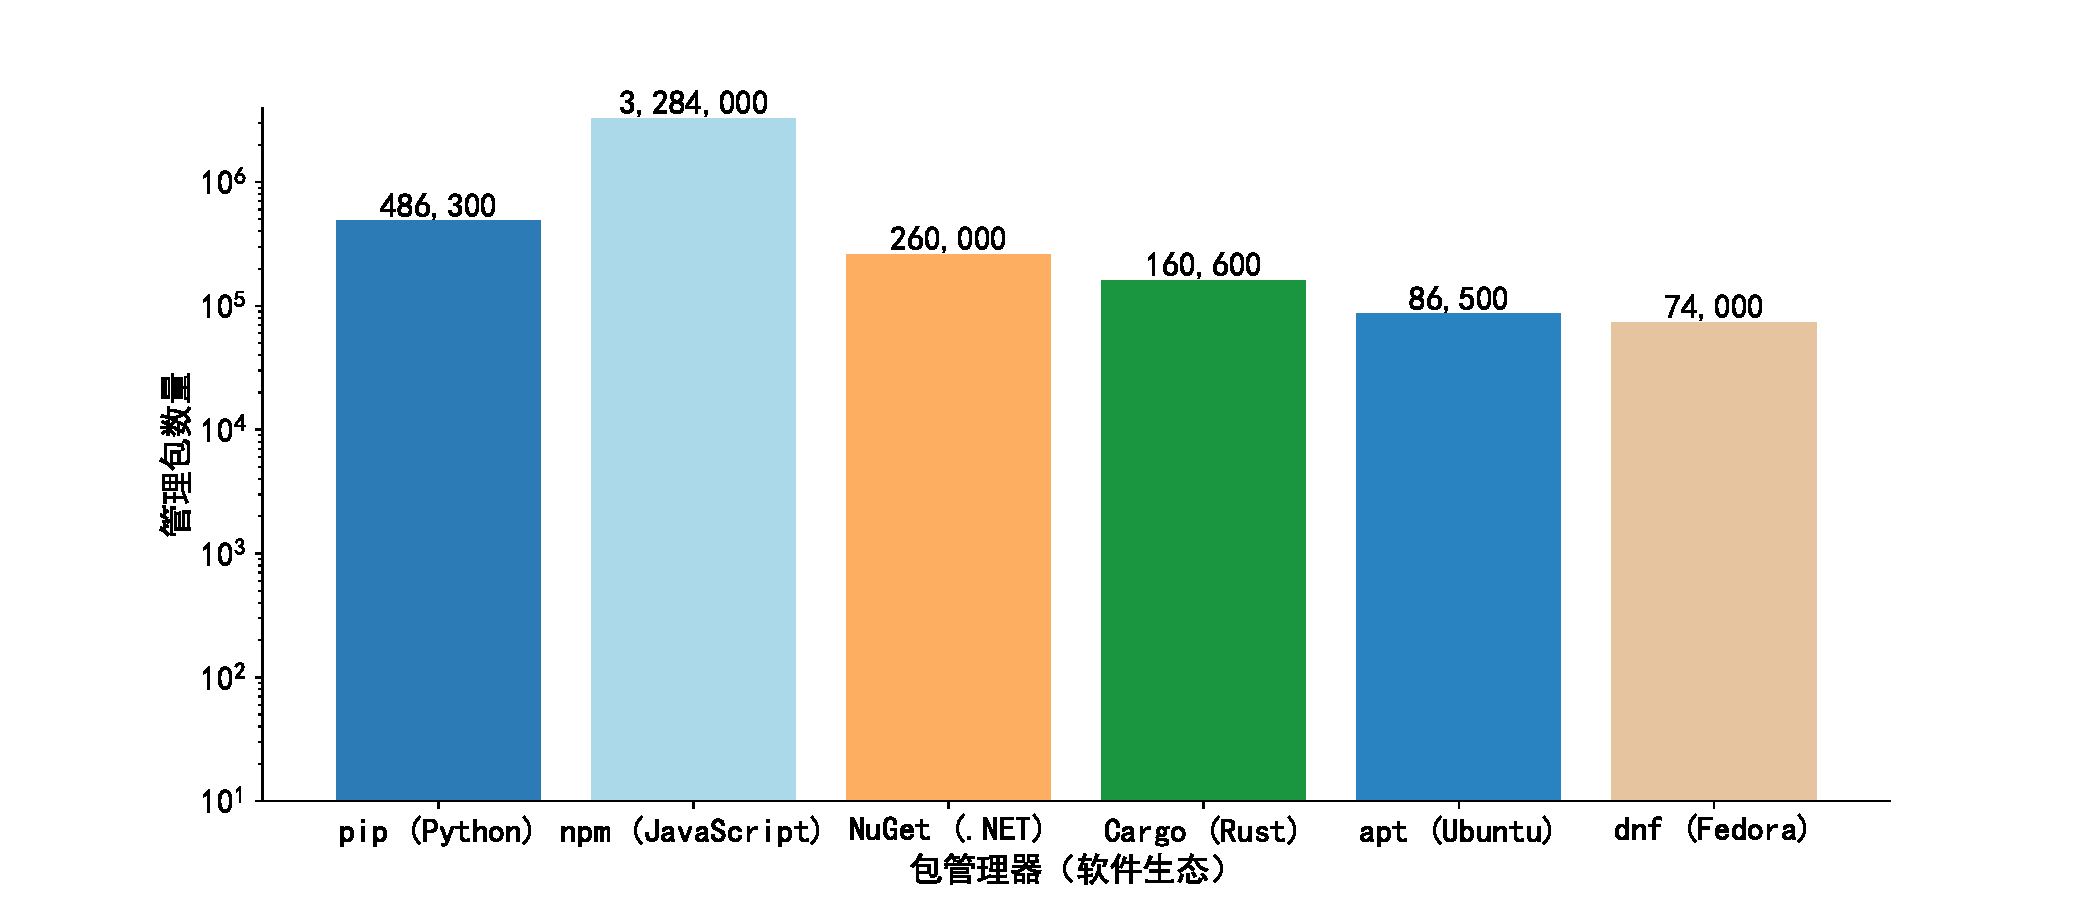
\includegraphics[width=0.96\textwidth]{background}
	\caption{不同软件生态的包管理器管理第三方包数量}
	\label{fig:bac}
\end{figure}

包管理工具的核心设计目标是确保在其对应的软件生态系统内,正确解析第三方包依赖关系,从而避免用户安装的第三方包之间发生不兼容的问题。为了实现这一目标,学术界中也有大量研究致力于提升第三方包的依赖管理和兼容性检测能力。在Python软件仓库方面,一系列研究工\upcite{bommarito2019empirical,wang2022smartpip,wang2020watchman,lieasypip}专注于增强包管理工具的依赖解析功能和兼容性检测。同样,JavaScript软件仓库的依赖管理也成为研究焦点,涌现了一些重要的工作\upcite{javan2023dependency,zerouali2018empirical,patra2018conflictjs}。此外,操作系统发行版社区软件仓库中的第三方包兼容性问题也受到了关注,相关研究如\upcite{artho2012software,abate2020dependency,claes2015historical,trezentos2010apt}提供了深入的洞见。

然而,尽管单个软件仓库内部的包兼容性通过这些工具和研究得到了一定的保证,但仅限于单个仓库的兼容性管理并不能完全解决系统整体的包兼容性问题。在实际的软件开发过程中,开发者往往需要依赖多个软件仓库的资源,这种跨仓库的资源使用带来了额外的第三方包兼容性问题,本文将这类问题称为跨软件生态的兼容性问题(cross-ecosystem compatibility,简称为\textbf{CC}问题)。目前,现有的包管理工具和研究主要集中在提高特定软件仓库的管理和兼容性检测能力上,这些努力虽然改进了单一软件生态的包管理,但在多软件生态系统共存的情况下,它们通常无法有效地检测和修复CC问题。

在知名编程问答网站StackOverflow \upcite{StackOverflow} 和开源平台GitHub \upcite{GitHub}中,有许多开发者会报告CC问题并寻求帮助。例如Github平台中的gradio 项目的问题\#5154\upcite{gradio_issue_5154},开发者在配置项目时遇到了apt仓库的包“jinja2” 与pip仓库的包 “markupsafe” 之间的CC问题。开发者报告了问题并和其他开发者展开了广泛的讨论,却仍未分析出问题的根本原因,最终只能将所有相关的第三方包都重新安装并降低版本才配置项目成功。但这种方式CC问题并未被解决,而只是不影响当前项目的运行,可能会影响系统内其他项目的运行。

因此,开发者迫切需要一种能解决多个软件生态系统共同作用下的包兼容性问题的新方法。本文针对这一研究空白,首先针对CC问题进行了实证研究,深入分析了CC问题的根本原因和问题特征,并探讨了CC问题对于系统的影响。然后本文提出了解决CC问题的新方法并设计实现了自动化工具用于预测、检测和修复CC问题。CC问题的发现和解决不仅对于提高软件系统的稳定性和性能有着直接影响,还有助于减轻开发人员的工作负担,优化开发流程,降低因兼容性问题带来的风险和成本。


\section{相关研究现状}
第三方包兼容性问题是软件可靠性领域的一个重要的研究热点。近年来,越来越多研究工作关注第三方包兼容性问题,它们主要聚焦于三个方向开展研究,分别是第三方包依赖冲突诊断,第三方包兼容性检测和第三方包演化过程中的API不兼容更改检测。本节将详细介绍三个研究方向的相关工作,并分析现有工作的局限性。
\subsection{依赖冲突诊断研究}
第三方包依赖冲突指一个项目依赖了两个或多个第三方包的冲突版本,现有大量工作致力于研究单个软件生态中的依赖冲突问题。与本文最相关的研究包括 \textsc{smartPip} \upcite{wang2022smartpip}、\textsc{EasyPip}\upcite{lieasypip}、\textsc{WatchMan} \upcite{wang2020watchman}、\textsc{PyDFix}\upcite{mukherjee2021PyDfix} 和 \textsc{SnifferDog}\upcite{wang2021SnifferDog}。\textsc{WatchMan}、\textsc{smartPip} 和 \textsc{EasyPip} 旨在解决最流行的 Python 包管理工具 pip 无法解决的 Python 依赖冲突问题。\textsc{WatchMan} 首先总结了由于 pip 安装规则导致的依赖冲突问题的表现形式,并提出了一种用于持续监控 PyPI 生态系统中依赖冲突的工具。该工具通过收集各第三方包的元数据,并进行广度优先搜索,构建了项目依赖的完整第三方包依赖图。这个依赖图是一张有向无环图,其中节点表示不同的第三方包,节点间的有向边表示包与包之间的依赖关系,边的箭头指向被依赖的第三方包。在依赖图中,如果一个节点有多条有向边指向,那么该节点就是被多个包依赖的第三方包;通过分析其入边集合,匹配边之间的版本约束关系,如果这些约束的交集为空,则说明存在依赖冲突问题。
\textsc{smartPip} 揭示了在 \textsc{WatchMan} 发布后的新依赖解析策略下依赖冲突问题的新特征。他们的方法同样能够在不更改版本约束的情况下解决依赖冲突问题。\textsc{EasyPip} 用于自动检测和修复 Python 依赖声明文件中的问题,在定位依赖冲突问题的根本原因方面比 \textsc{smartPip} 更加有效。然而,它们仅限于单一的软件仓库,未考虑受多个包管理工具影响的依赖冲突问题,也无法解决CC问题。\textsc{PyDFix}旨在解决 PyPI 上某些软件包由于环境兼容性问题而无法正确安装的问题。然而,CC问题通常不会在安装阶段发生,而是在项目的运行阶段发生。\textsc{SnifferDog} 通过模块信息和依赖信息修复 Jupyter Notebook 项目的环境,但未处理系统 Python 环境的问题。

除此之外,许多研究集中在其他生态系统中的依赖冲突问题上\upcite{li2022nufix,wang2018dependency,wang2019could,wang2021will,patra2018conflictjs,huang2020interactive}。例如,一些研究 \upcite{wang2018dependency,wang2019could,wang2021will,huang2020interactive} 主要关注 Java 生态系统中的依赖管理问题。他们发现,Maven \upcite{Maven}中的依赖冲突问题不会导致构建失败,但可能会引发语义行为不一致 \upcite{wang2021will} 或运行时异常 \upcite{wang2018dependency}。基于这一发现,一些研究者提出使用静态分析\upcite{wang2018dependency} 和动态分析 \upcite{wang2019could,wang2021will} 来识别 Maven 中的依赖冲突问题。对于 .NET 生态系统,Wang 等人对 NuGet\upcite{NuGet} 中的依赖冲突问题进行了实证研究。他们总结了表现模式和修复策略,并提出了一个有效的工具 NuFix \upcite{li2022nufix},通过调整版本约束来修复依赖冲突问题。\textsc{ConflictJS}\upcite{patra2018conflictjs} 针对 JavaScript 生态系统中的依赖冲突问题,因为第三方库共享同一个全局命名空间。

尽管以上这些研究在第三方包依赖冲突诊断领域取得了显著进展,但它们大多仅限于特定的软件仓库内部,没有全面考虑在多个包管理工具共同作用下可能出现的依赖冲突问题,也未能解决跨生态系统的复杂依赖关系所导致的兼容性问题。
\subsection{兼容性问题检测研究}
目前,在检测项目或第三方库之间的兼容性问题时,现有的解决方案主要依赖于比较不同版本第三方库的运行结果,或者通过构建项目的依赖关系图或抽象语法树来分析调用关系。Foo 等人\upcite{sakti2014instance}开发了 JTEXPERT,这是一种自动化的软件测试数据生成工具,旨在实现高代码覆盖率的单元测试。JTEXPERT 基于遗传算法,结合类实例生成器和种子策略进行优化搜索,并通过静态分析从搜索空间中排除不相关的输入变量,以加速搜索过程。生成的测试数据可用于检测不同版本第三方库及其调用关系中的不一致性。

开发者期望加载的版本与实际加载的版本不一致时,即使方法签名相同,程序行为也可能不同,这是一种常见的兼容性问题。为了解决 API 之间的兼容性挑战,Wang 等人\upcite{wang2021will} 提出了名为 SENSOR 的方法,利用遗传算法进行处理。SENSOR 首先从源代码中提取构造函数和 API 调用上下文,建立类实例池和 API 参数池。随后,使用 \textsc{GUMTREE}\upcite{falleri2014fine} 迭代检测代码差异,细粒度地识别出冲突的 API 对。通过将类实例的种子策略与 \textsc{EVOSUITE}\upcite{fraser2011evosuite} 相结合,SENSOR 生成了一组测试用例,用于触发不同版本的库 API,并检测其行为是否一致。

\textsc{PYCOMPAT}\upcite{zhang2020python} 通过静态分析来检测 Python 第三方库中因 API 变更引起的兼容性问题。具体而言,该工具用于识别 API 和参数的重命名问题,分为两个阶段进行:第一步,从第三方库提取 API 变更信息,若无法自动获取,则采用手动方式;第二步,以 API 知识库为输入,对 Python 源代码进行静态分析,生成抽象语法树(AST),遍历 AST 以识别框架定义的 API 调用,并通过预设的匹配规则检查是否使用了已修改的 API,从而定位兼容性问题。
Foo 等人\upcite{foo2018efficient} 则利用静态分析检查第三方库升级后是否引入了不兼容的 API 方法。他们首先构建程序的库调用图,使用 \textsc{Myers} 算法比较库升级前后的 API 差异,评估相近版本之间的 API 变化,得出差异结果。然后,结合依赖调用图评估不兼容的变更,并通过分析配置文件,推荐变动最小的版本。

以上这些研究能够在一定程度上有效检测第三方包之间的兼容性,但是它们有效的必要条件是要确定第三方包之间的调用关系。而对于检测CC问题首要的难题就是要确定第三方包之间的调用关系,这使得现有工作无法解决CC问题。本研究首先通过问题根因分析和特征分析设计了CC问题中的第三方包调用关系识别方法,之后基于现有研究工作实现了兼容性检测。
\subsection{API不兼容更改研究}
兼容性问题主要体现于API之间的不兼容,调研第三方包演化过程中API不兼容更改分析的相关研究工作,可以为检测兼容性问题提供参考性意见。API 不兼容更改也被称为破坏性更改,第三方包演化过程中发生不兼容更改的API称为破坏性API。API不兼容更改主要有两种检测方法:测试\upcite{mezzetti2018type,moller2019model,chen2020taming}和程序分析 \upcite{horton2019v2,zhang2020python,chen2020taming,ponomarenko2012backward,jia2021depowl,brito2018apidiff,silva2017refdiff,du2022aexpy}。

\textsc{NoRegrets}\upcite{mezzetti2018type} 是一个回归测试工具,可用于判断 JavaScript 第三方软件包的更新是否影响了更新后的 API 的使用。\textsc{NoRegrets+}\upcite{moller2019model} 可以自动生成测试用例,以查找 JavaScript 第三方软件包中的不兼容更改。\textsc{DeBBI}\upcite{chen2020taming}通过测试和分析来检测 Java 软件包和项目之间的不兼容性。对于静态编程语言,研究\upcite{brito2018apidiff,silva2017refdiff,revapi,clirr,japicmp,SigTest} 主要集中在分析 Java API 和检测不兼容更改。对于动态编程语言,\textsc{V2} \upcite{horton2019v2} 基于 Python 程序崩溃信息检测不兼容更改。一些研究\upcite{zhang2020python,du2022aexpy} 使用规则检测 Python 第三方软件包演进过程中的不兼容更改。还有一些研究在二进制级别检测不兼容更改\upcite{ponomarenko2012backward,jia2021depowl}。

为了解决第三方库在多种编程语言中的向后兼容性问题,\textsc{Ponomarenko} 等人提出了一种新的自动检测方法 [34]。该方法在二进制级别上工作,不仅分析组件二进制文件中的符号,还通过比较从组件头文件提取的函数签名和类型定义,来验证向后兼容性\upcite{ponomarenko2012backward}。
Jia 等人同样提出了二进制级别的第三方包不兼容更改检测工具,可以检测第三方包演化过程前向和后向不兼容问题。这种二进制级别的兼容性检测相比于API级别的检测更细粒度也更准确 \upcite{jia2021depowl}。

以上研究在检测不兼容更改方面表现良好,但其中许多方法的开销较大。为了能够在用户系统内轻量级地解决CC问题,本研究构建了包含数千万API不兼容更改的数据库,使用现有检测方法的成本较大。因此,本研究设计了基于规则的API不兼容更改检测方法,以最小的开销检测大多数不兼容更改。

综上,现有相关工作主要聚焦于单个软件生态中的兼容性问题的分析、检测和解决,对于CC问题尚未有成熟的解决方案。因此,探究一种有效分析和检测CC问题的方法,具有相当的研究意义和实践意义。

\ignore{
\begin{table}[htp]
	\centering
	\begin{minipage}[t]{0.8\linewidth} % 如果想在表格中使用脚注,minipage是个不错的办法
		\caption[表 1.1 名称]{}
		\begin{tabular*}{\textwidth}{lp{10cm}}
			\toprule[1.5pt]
			{\hei 列1} & {\hei 列2} \\
			\midrule[1pt]
			&  \\
			& \\
			& \\
			& \\
			& \\
			& \\
			\bottomrule[1.5pt]
		\end{tabular*}
	\end{minipage}
\end{table}
}

\section{研究内容和主要贡献}
目前,许多编程语言和操作系统社区常常维护第三方包软件库并提供相应的包管理工具,以建立自己的软件生态。这些工具通常都经过精心设计,以处理生态软件库内的依赖关系,而不考虑库间的依赖关系。现有的相关研究也只关注了单个软件生态内部第三方包之间发生的兼容性问题,忽略了多个软件生态共同影响的第三方包兼容性问题。为了弥补这一研究空白,本研究从两方面研究CC问题:(1)CC问题是如何发生的以及发生时的特征是什么?(2)如何自动化预测、检测和修复CC问题?具体而言,本研究以Python语言和Ubuntu系统两个影响广泛的软件生态为代表,深入分析研究Ubuntu系统上不同仓库中Python第三方包出现的CC问题,总结CC问题的触发模式、故障症状和根本原因,在此基础上,本研究设计并实现对应的自动化检测工具,在解决Python语言和Ubuntu系统间的CC问题的同时,也对其他软件生态间的类似问题的研究起到启发和指导作用。
\subsection{跨软件生态兼容性问题实证研究}\label{1.3.1}
在Ubuntu系统中,用户管理Python第三方库最普遍的做法是利用包管理工具,包管理工具会在系统内维护一个本地仓库存储从对应软件源中安装的第三方包,其中最为广泛使用的第三方包管理工具是apt和pip。Apt是Ubuntu系统的官方包管理工具,可以帮助用户安装、更新和卸载各种语言的第三方包,其中包括数千个Python第三方包。Pip是Python语言最常用的包管理工具,其软件源是PYPI,存储了数百万个Python第三方包。对于用户而言,使用apt安装Python包可以确保系统级别的包依赖关系得到正确处理(例如Python第三方包和一些二进制库之间的兼容性),而使用pip则可以安装种类更多版本更丰富的Python。因此,用户在实际开发中,往往需要同时使用apt和pip安装Python第三方包,从而兼顾系统的稳定性和开发的灵活性。然而,本研究发现系统内不同软件仓库中的第三方包会发生CC问题,并且CC问题在包管理工具安装第三方包时不会被检测到。那么,CC问题为什么会发生以及CC问题为什么现有的包管理工具无法检测到呢?

为了回答上述问题,本研究从CC问题的根本原因,问题特征和问题影响三方面展开了实证研究。在CC问题的根本原因方面,本研究从两方面入手分析原因,首先,从Python包安装策略来看,apt和pip的策略迥然不同,apt只检查自身仓库依赖关系并安装对应操作系统固定版本的包,pip会检查系统内全部的包并安装符合约束的最新版本的包,这会导致apt仓库和pip仓库中安装同一个Python第三方包的不同版本。其次,从Python解释器导入Python包策略来看,解释器会按照包名根据固定顺序在系统各个包仓库中搜索Python第三方包,如果找到则不搜索其他目录,这会导致解释器会从不同仓库中导入一个包和它的依赖包。基于上述分析,本研究总结了CC问题的根本原因。

在CC问题的问题特征方面,本研究从GitHub和Stack Overflow收集并筛选处出27个真实世界CC问题,并进行了详尽的分析,最终总结了CC问题的问题特征,包括三种触发模式和四种故障症状。与此同时,在总结CC问题特征时,本研究发现每个CC问题都包含一个应用包和一个库包。应用包通常托管于apt仓库中,而库包则同时托管于apt和pip仓库中(应包用和库包是相对概念,因为一个应用包本身可能是另一个应用的库包)。这一发现揭示了两种关系:(a)应用包与托管于apt的库包是兼容的;(b)托管于apt的库包与pip中的同名库包不兼容。例如章节\ref{3.1.1}中的图\ref{fig:example}中的“amp 0.6.1”是一个应用包,“scipy 1.3.3”,“numpy 1.17.4”和“numpy 1.24.3”是库包,其中两个库包“numpy”分别托管于apt和pip仓库且二者不兼容。

在CC问题的问题影响方面,本研究基于最常见的一种触发模式,通过大规模的测试和分析,研究了CC问题对于Ubuntu20.04系统的影响。具体而言,本研究首先从Ubuntu20.04系统的apt软件仓库中的全部Python包出发,结合依赖关系和PyPI软件仓库中的Python包,构建了23866个可能出发CC问题的包安装指令序列。然后,本研究逐一测试安装序列,发现由1692个序列会发生CC问题.本研究收集这些问题的错误信息以构建一个CC问题数据集,这些CC问题导致原本可以正常导入的Python第三方包导入失败。在实际用户环境中,这些失败可能会导致正常运行的系统软件崩溃,并且CC问题发生时的错误信息和传统包兼容性问题类似,导致用户难以排查并解决问题。这些实证研究的结论,为后续设计自动化解决工具提供了基础。
\subsection{跨软件生态兼容性问题的预防、检测和修复}
为了提升Ubuntu系统中的Python依赖包治理能力,本研究致力于自动化解决CC问题,本研究设计了一种自动化工具\tool{}\footnote{CC问题发生在来自两个软件生态的Python第三方包间,作者联想到了“双头蛇”,而在希腊神话中Hera饲养了一条双头蛇,因此将本研究提出的工具称为\tool{}。}来预测、检测和修复CC问题。对于预测CC问题,当用户执行安装命令时,\tool{}
预测这些命令是否会导致CC问题。对于检测CC问题,\tool{}会扫描用户系统中安装的所有Python包,并检测是否存在CC问题。对于修复CC问题,当检测到CC问题时,\tool{}会提供修复建议,防止用户出现故障。
由于这三种情况都在用户的生产环境中工作,因此在部署\tool{}时,开销应至关重要。在这方面,\tool{}的核心在于离线建立一个兼容性数据库,然后在线预测、检测和修复CC问题。离线阶段和在线阶段都具有挑战性:
\begin{itemize}
	\item \textbf{构建跨软件生态的兼容性数据库较为困难。}软件生态的软件仓库可能包含大量软件包(例如,pip目前管理着近五十万个软件包),其中大多数软件包具有较长的演化历史。这些软件包不断进行异步演化,因此数据库也必须相应地不断更新。来自不同仓库的软件包之间的依赖关系组合将是巨大的。考虑所有可能的软件包版本组合几乎是不可能的。
	\item\textbf{ 预测、检测和修复CC问题并非易事。}每个软件生态的软件仓库都有其独特的管理工具,并采用不同的安装策略和目录结构。安装软件包时,若apt在其自身的安装目录中找不到该软件包,则会安装操作系统发行版预先设定的版本,而pip则会在系统级目录中找不到该软件包时安装最新版本。导入软件包时,Python解释器会按照预定义的顺序依次检查所有目录。CC问题涉及以上三者(即 apt、pip和Python解释器)之间的交互,使其难以预测、检测或修复。
\end{itemize}

为了解决第一个挑战,基于章节~\ref{1.3.1}对于CC问题的分析研究,鉴于此,\tool{}在兼容性数据库中创建了两个表:
\begin{itemize}
	\item \textbf{依赖表}:对于apt仓库中的每个应用包,该表收集其对apt仓库中各个库包的API使用情况。
	\item\textbf{兼容性表}:对于apt仓库中的每个库包,该表收集其与pip仓库中不同版本的同名库包的API兼容性。
\end{itemize}
这两个表提供了有关CC问题的充分信息,并且其规模是可接受的,因为apt仅管理约3,319个操作系统发行版预先设定的版本的Python软件包。当操作系统发行版发布时,\tool{}会构建一个新的数据库。之后,\tool{}会增量地获取pip仓库中的最新软件包版本。

针对第二个挑战,本研究提出了系统级软件包依赖图(S-PDG),用于描述apt、pip和Python解释器之间的交互关系。S-PDG 包含用户系统中所有 Python 软件包的依赖关系。为实现这一点,\tool{}首先分别构建了由 apt 和 pip 安装的软件包的两个依赖图。我们将这两个依赖图称为仓库级软件包依赖图(R-PDG)。之后,\tool{}根据 Python 解释器的导入规则将两个 R-PDG 合并为一个 S-PDG。在检测场景中,当两个版本的相同库软件包出现在S-PDG 中时,\tool{}会查询兼容性表,以确定这些版本之间是否存在破坏性 API。如果存在破坏性 API,\tool{}会进一步查询依赖表,以检查系统中是否有使用这些破坏性 API 的应用程序包。如果有,Hera 会报告一个 CC 问题。在预测场景中,\tool{} 会试运行安装命令,然后将待安装的软件包临时添加到 S-PDG 中,然后重复和检测场景相同的过程。在修复场景中,\tool{} 可以根据 R-PDG 中的依赖关系提供修复建议,这些依赖关系被认为是兼容的,因为它们仅包含单个仓库内的依赖关系。

本研究对于\tool{}进行了广泛的实验评估,在章节~\ref{1.3.1}构建的CC问题数据集的23866个序列上,\tool{}检测到 3689 个 CC 问题,其精确度为 90.5\%。这些问题可以覆盖数据集中 1,692 个问题中的 93.7\%。为评估分析不兼容 API 变更的有效性,本研究手动检查了结果,发现其精确度和召回率分别为 91.1\% 和 98.2\%,置信水平为 95\%,误差范围为 5\%。本研究还复现了来自 GitHub 和 Stack Overflow 的 26 个真实世界CC问题,\tool{}能够检测到全部这 26 个实际CC问题,并提供准确的原因和修复建议。
\subsection{主要贡献}
总结而言,本文的主要贡献如下: 
\begin{itemize}
	\item \textbf{新的研究问题。}本研究首次系统地探讨了跨软件生态的兼容性问题,这是第三方包兼容性领域中的一个新问题。本研究定义了CC问题,并专注于从Python生态和Ubuntu生态的视角进行研究。具体而言,本研究针对CC问题进行了大规模的实证研究,最终总结了问题的根本原因,问题特征和问题影响。CC问题的研究不仅局限于Python,同样适用于其他编程语言和软件生态系统,本研究对于其他软件生态中类似问题的研究提供了启发和方向。
	\item \textbf{新型工具实现。}作为解决上述问题的一部分,本研究设计实现了一种新型工具\tool{},用于自动化解决CC问题。\tool{}的核心思想是离线构建一个兼容性数据库,并在线预测、检测和修复CC问题。\tool{}的设计考虑了实际应用中的需求,可以无缝地集成到用户的生产环境中,并且保持操作的轻量级,使得在大规模软件仓库中的应用成为可能。
	\item \textbf{广泛实验评估。}为了验证\tool{}的效果和实用性,本研究对其进行了广泛的实验评估。评估结果表明,\tool{}在 CC 问题检测中的精确度和召回率方面都具有良好的效果,工具中最关键的基于规则的API不兼容更改识别方法也具有高精度和高召回率。\tool{}还能够检测并修复来自 GitHub 和 Stack Overflow 的真实世界 CC 问题。
\end{itemize}
通过这些贡献,本研究不仅推动了对跨软件生态的兼容性问题的理解,还为实际应用中的问题提供了有效的技术解决方案。本研究还可以激励更多的研究和开发工作,进一步探索和完善跨生态兼容性问题的解决策略。

\section{论文结构}
本文组织分为五个部分,每部分的内容具体如下:

\textbf{第一章 绪论。}本章阐述了研究背景、研究意义、研究内容和贡献、以及论文的组织结构。首先,通过分析当前第三方包依赖和兼容性管理的挑战和机遇,明确研究的背景和问题。接着定义研究的主要内容和贡献,最后总结整篇论文的结构和各章节的主要内容。

\textbf{第二章 相关理论基础。}本章探讨了跨软件生态的兼容性问题的相关理论基础,涵盖了第三方包依赖管理和API不兼容更改等多个关键领域。在第三方包依赖管理方面,本章分析了不同包管理工具的依赖解析策略,并探讨了它们的优势和适用场景。在API不兼容更改方面,本章探讨了API不兼容更改对第三方包兼容性的影响,以及如何检测这些更改。这些相关理论基础为后续章节提供了理论背景和技术基础。

\textbf{第三章 跨软件生态的兼容性问题实证研究。}本章分析了在Ubuntu系统中使用apt和pip管理Python第三方包时出现的第三方包兼容性问题。通过实证研究,本章揭示了CC问题的成因、特征,并构建了包含1692个案例的CC问题数据库。本章总结的CC问题特征包括三种触发模式和四种故障表现,为后续设计有效的自动化解决工具提供了洞见。

\textbf{第四章 跨软件生态的兼容性问题预测、检测和修复。}本章探讨了 \tool{}的设计与实现,分别介绍了\tool{}在离线阶段如何构建一个兼容性数据库,在在线阶段如何检测和预测CC问题,以及图和提供修复建议。此外,本章还阐述了一套新的基于规则的方法来分析库软件包不同版本间的破坏性API更改,并详细描述该方法的过程。


\textbf{第五章 实验与评估。}本章深入阐述了实验的设置、执行过程以及结果分析。首先,介绍了实验的具体设置,包括数据来源、方法选择和评估标准。随后,通过大量实验验证了所提方法的有效性,并从不同角度对结果进行了详细分析。最后,对实验结果进行了深入讨论。

\textbf{第六章 总结与展望。}本章对全文的主要研究内容和贡献进行了总结,并展望了未来的研究方向。首先,概括了本文的关键发现和贡献;然后,基于当前研究现状和本研究结果,探讨了未来可能的研究方向和挑战。最后,对全文内容进行了梳理和总结。



\chapter{相关理论基础}
本章介绍了本研究的相关理论基础,这些理论基础支撑了本文后续的实证研究和工具设计。本章首先介绍了第三方包依赖管理,阐述了三种依赖解析策略并分析了不同包管理工具的优势和使用现状。随后,本章详细探讨了API不兼容更改导致的第三方包兼容性问题,并介绍相应的检测技术。接下来,本章从静态分析和动态分析两方面介绍了程序分析技术,这些技术部分应用于本文的工具实现,是有效检测CC问题的技术基石。

\section{第三方包依赖管理}
\subsection{依赖解析}\label{2.1.1}
在软件生态中使用某个第三方包时,项目需要指定所需包的版本约束条件。找出满足指定版本约束条件的每个所需包的适当版本的过程称为“依赖解析”。根据版本约束的解决方式,本研究将现有的包管理器分为三类。

第一类采用迭代方式来计算可行解。具体而言,每次它首先搜索并下载一个满足版本约束条件的目标包$P_{i}$的版本,然后迭代地验$P_{i}$的每个直接依赖包的版本约束是否得到满足。Pip、poetry\upcite{Poetry} 和 pipenv 是这一类别的代表性工具。

第二类将所需包的版本约束编码为一个 SAT 求解问题,然后借助求解器直接计算每个所需包的适当版本。本质上,如果存在满足所有所需包版本约束的可行解,这种技术方案不会导致因依赖冲突而引发的构建失败。这一类别的代表性工具是 Conda\upcite{Conda}。然而,由于将依赖解析编码为 SAT 问题的复杂性,Conda 长期以来一直受到性能问题的困扰,这在其问题报告系统中已被广泛讨论\upcite{Issue7239,Issue8197,Issue8810,Issue9983,Issue11414}。此外,Conda 开发者也承认,Conda 在依赖解析方面通常比 pip 慢\upcite{Issue7239}。

第三类是固定版本策略。在以Linux发行版为代表的操作系统生态中,为了维持系统的安全性和稳定性,往往会在系统发布时维护一个版本固定的第三方包列表,每个第三方包有且只有一个版本并且各个包之间相互兼容。在此基础上,这类生态的包管理器只需检索列表安装固定版本的第三方包及其依赖包,即可避免依赖冲突问题,Ubuntu系统上的apt是此类工具的代表。

\subsection{包管理工具分析}
本研究以Python语言和Ubuntu系统两个影响广泛的软件生态为代表,研究Ubuntu系统上不同仓库中Python第三方包出现的CC问题,其中不同仓库指的是Ubuntu系统的apt包管理工具维护的第三方包仓库(本文中简称apt仓库)以及Python语言的pip包管理工具维护的的第三方包仓库(本文中简称pip仓库)。在本节中将分析这两种包管理工具安装Python包的各自优势以及用户的使用现状。

在Ubuntu系统中,Python软件包管理是系统软件依赖管理中的关键组成部分。Ubuntu以其强大的包管理工具apt而闻名它为系统提供了方便的软件安装、升级和卸载功能。同时,Python生态也有其专用的包管理工具pip,负责下载、安装和管理Python相关的软件包。在Ubuntu系统上,apt为Python软件包提供了全局的系统级别管理。这意味着通过apt安装的软件包将被整合到系统的共享库和依赖项中,为所有用户和应用程序提供一致的运行环境。使用apt管理python依赖有以下优势:
\begin{itemize}
	\item \textbf{系统级别的依赖。}Uubuntu 系统中的一些应用程序和工具依赖于特定的 Python 包(例如:Fail2ban)。Apt 能够管理这些系统级别的依赖,确保在安装、更新或卸载这些应用程序时,相关的 Python 包也会被正确处理并且可以确保系统级别的依赖关系得到正确处理。
	\item \textbf{安全性和稳定性。}Apt提供的python包都是经过严格审核测试的,可以确保这些包的安全性,而pip安装的包有可能有安全性问题。与此同时,如章节\ref{2.1.1}所说,apt仓库中的Python包通常与Ubuntu 系统版本相匹配,这有助于确保系统的稳定性。
	\item \textbf{处理非Python依赖关系。}当一个 Python 包依赖于其他非 Python 的系统库时,使用 apt 可以更好地管理这些依赖关系。Apt 包管理器会确保所有必要的依赖项被正确安装和管理。例如,LXML 是一个 Python 库,它依赖于 libxml2 和 libxslt 等 C 库。通过使用 Apt 安装 python3-lxml,可以确保这些库也被正确安装。
\end{itemize}

然而,apt只能下载数千个流行python包,当开发者需要安装其他python包时,则需要使用其他方式。Pip是开发者最流行使用的python包管理工具,可以从Python包索引(PYPI)中下载数百万python第三方包,给用户提供了极大的灵活性。Pip支持安装包及其依赖关系、版本控制和包的升级。它允许用户从一个命令行界面轻松地管理包,使得Python开发和部署更为简便。Pip 还支持从本地文件、版本控制或直接从 URL 安装包,提供了高度的灵活性和控制,是 Python社区中不可或缺的工具之一。

除了上述包管理工具之外,目前的Python项目环境配置中还有一种常见的方式是构建虚拟环境。Python虚拟环境是一种独立的目录树,包含了一个Python解释器以及一系列附加的包。使用虚拟环境可以在不影响全局Python安装的情况下,为不同项目安装不同版本的库。这种隔离的环境使得项目依赖更加清晰,避免了不同项目间依赖包版本冲突的问题。Python可以通过venv模块或者Conda工具创建、管理虚拟环境,使用简单的命令就可以激活或停用特定的虚拟环境。这样,开发者可以在各自独立的环境中开发和测试应用,确保项目的稳定性和可复现性。然而在一些情况下用户应该使用apt安装Python包而不是构建虚拟环境:
\begin{itemize}
	\item \textbf{操作系统工具和服务。}许多Ubuntu会使用 Python 编写的系统工具和服务。在这种情况下,这些工具和服务的依赖关系需要在系统级别进行管理,因此使用 apt 安装相关的 Python 包是更好的选择。例如,Ubuntu 的系统更新管理器 update-manager 依赖于 Python,这时候使用 apt 来安装和管理这些依赖关系是合适的。
	\item \textbf{需要特定包版本的应用。}当一个应用程序依赖于特定版本的系统包时(例如,需要与系统的其他组件共享包),使用 apt 可以确保包文件和应用程序之间的兼容性。例如,如果正在使用一个需要特定版本的 GTK+ 库的 Python 图形界面应用程序,那么使用 apt 安装 Python 的 GTK+ 绑定(如 python3-gi)可能是更好的选择。
\end{itemize}

综上所述,在Ubuntu系统中,用户同时使用apt和pip在系统环境中管理Python第三方包是一种正常而必要的实践,这种方式可以充分利用两者的优势,确保系统稳定性和灵活性的平衡。但由于二者的设计目标是处理生态软件库内的依赖关系,而不考虑库间的依赖关系,给CC问题的发生提供了条件。

\section{API不兼容更改}
在本文中,API(应用程序编程接口)指的是第三方包对外提供和暴露的调用接口,在Python第三方包中,包括类、函数和属性等。APT不兼容更改指第三方包在演化过程中引入的不兼容的改变(例如改变函数接口签名)。其他第三方包(应用包)使用包含不兼容接口的第三方包版本(库包)会导致发生错误,本文称之为兼容性问题。

\subsection{API不兼容更改分析}
第三方包兼容性问题通常涉及三方参与者:库包开发者、应用包开发者和终端用户。在本文中应用包和库包是一对相对概念,一个应用包可能是另一个应用包的库包。
\begin{figure}[t] % use float package if you want it here
	\centering
	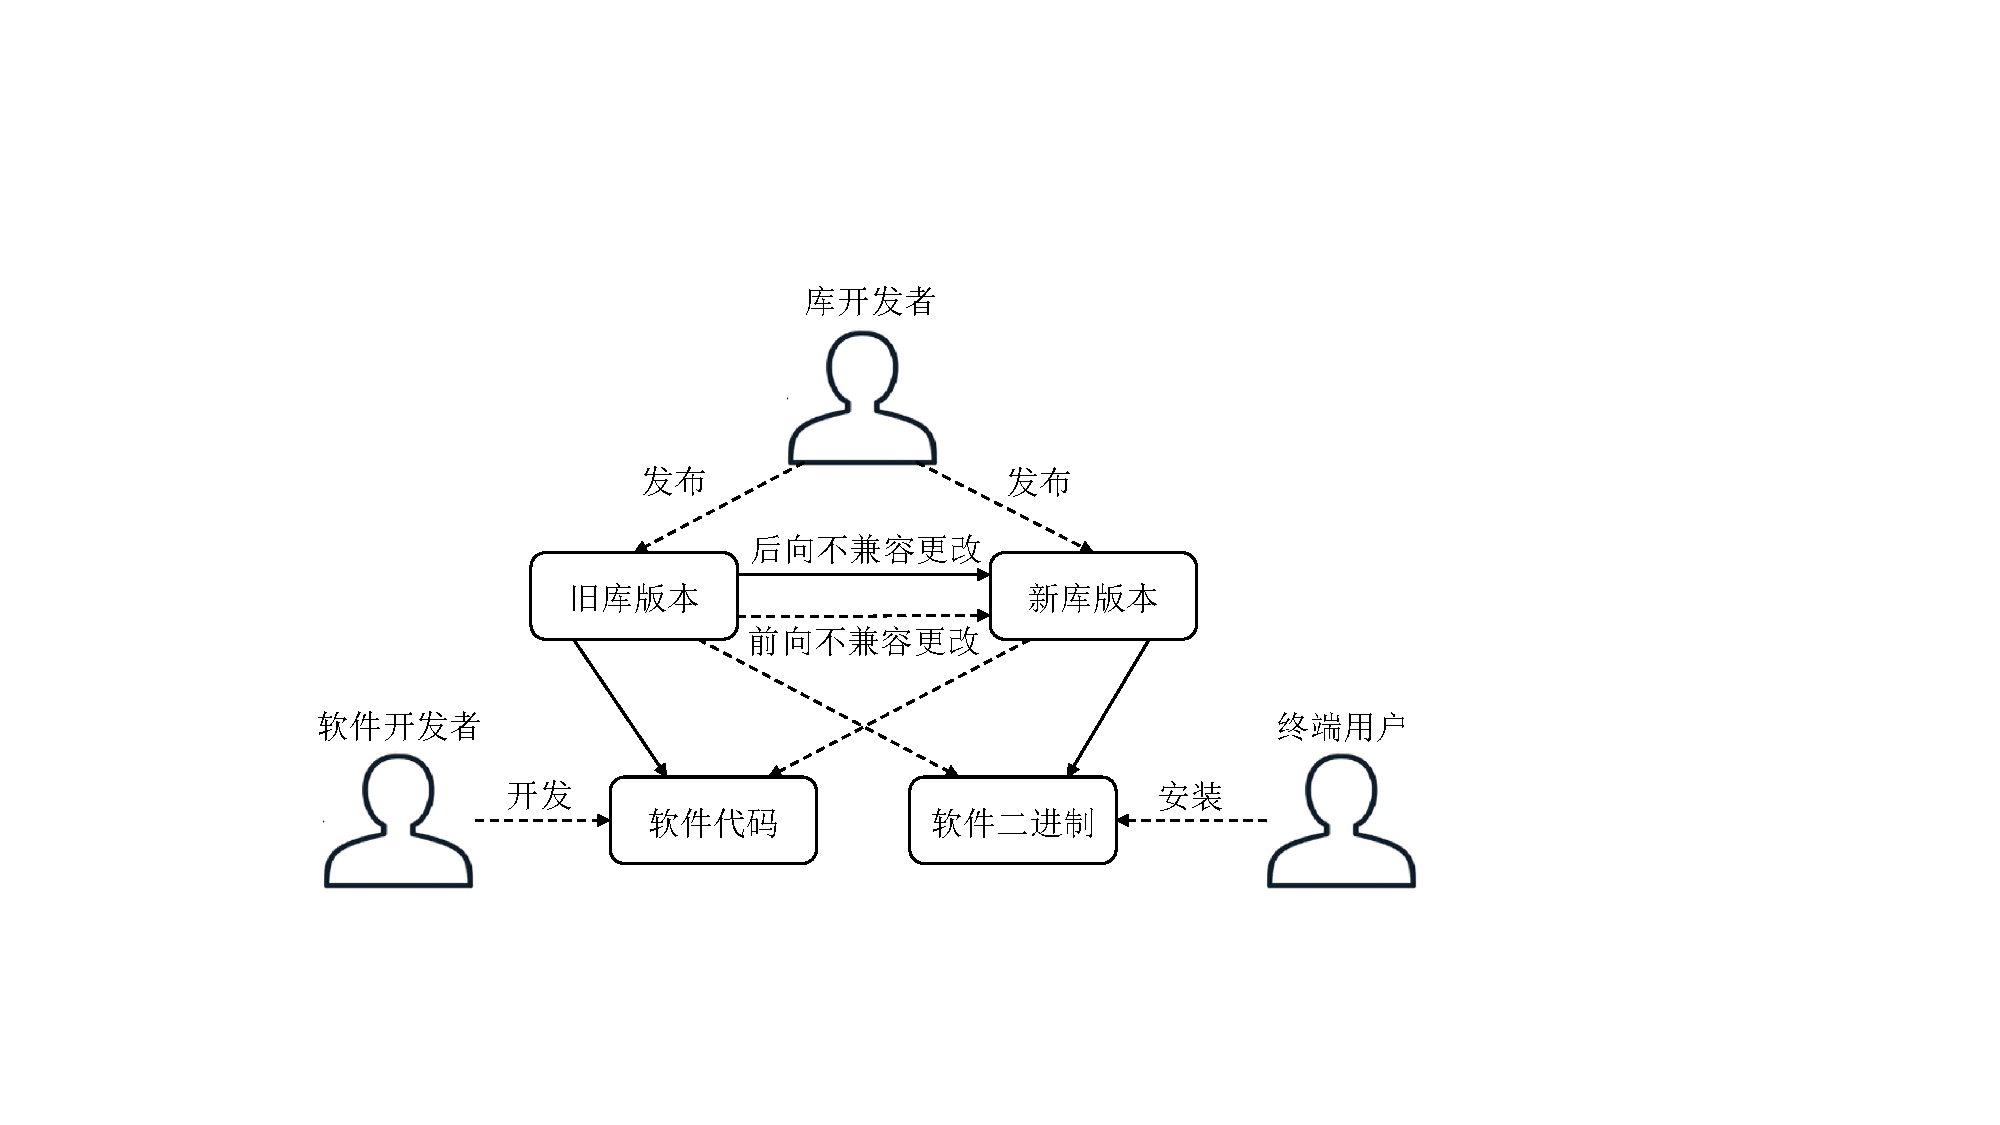
\includegraphics[width=5in]{API不兼容}
	\caption{API不兼容更改导致第三方包发生兼容性问题}
	\label{fig:API}
\end{figure}
图\ref{fig:API}中描述了由于 API 不兼容更改引起第三方包兼容性问题的两种情况。首先,库包开发者发布了两个包含不兼容更改的版本,这些更改分为两类:前向不兼容更改(例如添加一个函数接口)和后向不兼容更改(例如删除一个函数接口)。图中的实线代表了后向不兼容更改导致包兼容性问题的过程:即应用包开发者基于旧版本的库包进行开发,而终端用户在运行时将应用包链接到新的库包版本。类似地,图中的虚线表示前向不兼容更改导致包兼容性问题的过程:也就是应用包开发者基于新的库包版本进行开发,而终端用户在运行时将应用包链接到旧的库包版本。

当第三方包出现不兼容更改时,上述三类参与者可以采取不同策略来避免兼容性问题:1)库包开发者在最新版本中撤销不兼容的更改;2)应用包开发者更新应用包以适应库包的变化;3)终端用户避免使用不兼容的库包版本。许多研究致力于检测第三方包的变更\upcite{brito2018apidiff,foo2018efficient,meng2012history,mezzetti2018type,ponomarenko2012backward,wu2010aura},并将其报告给库包开发者(即采用第一种方法解决)。另外,一些研究关注于检测软件对不兼容 API 的使用\upcite{he2018understanding,jezek2013software,li2018cid,wang2019could},或协助软件适应库包的变化\upcite{balaban2005refactoring,henkel2005catchup,perkins2005automatically,xing2007api}。这些技术可以帮助应用包开发者更新应用包(对应于第二种方法的解决方案)。然而,在上述两种情形中,终端用户已经受到第三方包兼容性问题的影响,并且需要等待库包或应用包发布新版本。相比之下,第三种策略更加轻量化:终端用户从一开始就避免使用不兼容的库包版本,从而规避兼容性问题\upcite{贾周阳2020}。

在本研究中,本文基于这三种解决方案的相关研究工作,通过检测库包间的不兼容API和应用包对于库包不兼容API的使用,构建兼容性数据库进而支持终端用户避免使用不兼容的库包版本。

\subsection{API不兼容更改检测}
API不兼容更改检测是一个关键的第三方包维护活动,旨在识别和评估由于API更新而可能导致的兼容性问题。这种检测通常涉及到分析API的历史版本与新版本之间的差异,以确定哪些更改可能会破坏依赖于这些API的现有应用包。有效的API不兼容更改检测可以帮助终端用户避免潜在的第三方包兼容性问题。

API不兼容更改检测可以通过多种技术和工具来实现,主要包括静态分析和动态分析两种方法。静态分析和动态分析是根据代码是否在执行过程中进行分析来区分的。静态分析不涉及程序的运行,它通过分析代码或二进制文件来检测问题。这种方法可以覆盖代码的所有潜在执行路径,但可能会产生较多的误报。相比之下,动态分析在程序运行时进行,能够实时检测程序的行为,这使其更加有效地识别出实际运行中可能出现的漏洞。然而,它也有局限性,可能无法发现在当前测试环境下未被触发的潜在漏洞。在静态分析方面,主要有以下三种方式进行分析:
\begin{itemize}
	\item \textbf{签名比较。}通过比较API的签名(如方法名称、参数类型、返回类型等)来识别API不兼容更改。这种方法可以快速发现显著的改变,如方法的移除或参数的修改。
	\item \textbf{代码模式分析。}分析API实现的代码模式变化,如算法逻辑的变动或状态条件的修改。
	\item \textbf{依赖树分析。}分析应用包的依赖关系,确定哪些应用包代码可能受到API不兼容更改的影响。
\end{itemize}
在动态分析方面,主要有以下两种方式进行分析:
\begin{itemize}
	\item \textbf{回归测试。}运行旧版本API的测试套件对新版本进行测试,查看是否存在功能回归。
	\item \textbf{行为比较。}通过模拟或实际执行两个版本的API来比较其运行时行为的差异。
\end{itemize}

在后续的研究中,本文设计了一种自动化解决CC问题的工具\tool{},其中关键的一部分是构建跨软件生态的兼容性数据库,数据库中包含两个表格,分别为(1)依赖表:对于apt仓库中的每个应用包,该表收集其对apt仓库中各个库包的API使用情况和(2)兼容性表:对于apt仓库中的每个库包,该表收集其与pip仓库中不同版本的同名库包的API兼容性。\tool{}基于静态分析技术,实现分析应用包中对库包API的使用。\tool{}结合静态分析和动态分析技术,实现分析apt仓库和pip仓库中不同版本的同名库包的API兼容性。

\section{程序分析}
程序分析是软件开发中用于评估和改善程序代码兼容性、性能和可靠性的关键技术。通过深入分析代码,开发者可以确保不同软件组件之间的顺利交互,并减少运行时错误。这种分析通常分为两大类:静态分析和动态分析,每种方法针对不同的分析需求提供独特的视角和技术。

\subsection{静态分析}
静态分析是在程序执行前对代码进行的分析,目的是在不运行程序的情况下发现可能的错误和兼容性问题。它依赖于对代码的深入理解和自动化检查,能够覆盖代码的所有可能执行路径。静态分析通过分析程序的源代码、字节码或二进制执行文件,预测程序在运行时可能的行为。它不涉及程序代码的实际执行,而是利用各种算法和模型来模拟程序执行的结果。静态分析主要有以下关键技术:抽象语法树,数据流分析,控制流分析和符号执行。

\textbf{抽象语法树:}抽象语法树(AST)是源代码的树状表示,用于表达程序结构的层次关系。每个节点代表程序中的一个构造,如表达式、语句或声明。静态分析工具通过遍历AST,能够详细检查代码的每个元素,评估其对整体程序行为的影响。AST是实现代码优化、复杂度分析和代码重构等功能的基础。通过精确分析AST,可以精确地识别出代码中的逻辑错误、不兼容的API调用和潜在的安全漏洞。

\textbf{数据流分析:} 数据流分析通过跟踪程序中各变量的定义和使用来识别潜在的代码缺陷,如未初始化的变量、冗余的代码或潜在的空指针引用。这项技术不仅检测错误,还能优化编译器的代码生成,提高程序的运行效率。

\textbf{控制流分析:} 控制流分析涉及构建和分析程序的控制流图(CFG)。CFG帮助分析程序的执行路径,检测死循环或不可达代码。此外,通过对CFG的详细分析,可以优化程序结构,改进代码执行路径,从而提升程序性能。

\textbf{符号执行:} 符号执行是一种强大的静态分析技术,它使用符号值而非实际数据执行程序。通过这种方式,分析者可以探索程序的所有可能执行路径,检查路径特定条件下的程序行为。这不仅能发现难以通过常规测试触发的错误,还能帮助验证程序中的安全策略和业务逻辑。

静态分析有许多应用实例,本节介绍两类代表性应用。(1)代码兼容性检查:静态分析工具如 ESLint、SonarQube 专门用于检查代码兼容性问题,确保代码遵循最新的编程标准和兼容性指南。这些工具可以集成到持续集成/持续部署(CI/CD)管道中,自动检测提交的代码是否满足预设的质量标准。(2)漏洞识别:工具如 Fortify 和 Coverity 通过静态分析识别常见的安全漏洞,例如跨站脚本(XSS)和SQL注入。这些工具使用先进的模式匹配和数据流分析技术来检测可能被攻击者利用的代码弱点。

\subsection{动态分析}
动态分析在程序运行时进行,直接分析程序的执行行为。通过监控程序执行,动态分析提供关于程序实际运行状态的直接数据,这对于性能调优、错误诊断和验证软件行为尤其重要。动态分析涉及在程序运行时收集关于其行为的信息。这种分析依赖于程序的实际执行,可以利用测试用例或在生产环境中监控程序。动态分析主要有以下关键技术:代码覆盖率分析,性能分析,异常监测和追踪和日志记录。

\textbf{代码覆盖率分析}: 通过测量在程序测试过程中实际执行的代码部分,代码覆盖率分析帮助评估测试的全面性和效果。这不仅提供了测试的定量评估,还指导开发者优化测试案例,确保重要的代码路径得到充分测试。

\textbf{性能分析:} 性能分析工具如 Profiler 分析程序的执行时间和资源消耗,识别性能瓶颈。通过详细的运行时数据,这些工具可以帮助开发者了解程序在不同条件下的表现,并指出优化的具体方向。

\textbf{异常监测:} 动态分析工具实时捕获程序运行时的异常和错误,提供关键的故障诊断信息。这些工具通常能够追踪到异常发生的具体位置和条件,大大缩短了问题定位和修复的时间。

\textbf{追踪和日志记录:} 追踪程序的执行轨迹,记录详细的运行时数据,帮助开发者了解程序行为和出现问题的环节。这些数据对于后续的程序优化和错误预防具有重要价值。

静态分析也有许多应用实例,本节介绍两类代表性应用。(1)性能优化:动态分析工具如 New Relic 和 Dynatrace 在生产环境中监控应用程序的性能,提供实时性能优化建议。这些工具的洞察帮助开发团队快速响应性能问题,保证应用程序的高效运行。
(2)实时错误跟踪:工具如 Sentry 和 Bugsnag 在应用程序运行时监控错误,提供即时反馈和修复支持。这些工具的实时错误跟踪功能对于维护复杂的生产环境非常关键,帮助团队减少应用宕机时间和提高用户满意度。

结合静态和动态分析为代码兼容性提供了全面的保障。静态分析提前发现潜在错误和兼容性问题,而动态分析补充实际运行时的观察,两者相结合,使开发者能够更全面地理解和优化软件。这种综合方法不仅提升了软件的质量和性能,也增强了代码的兼容性和可维护性,是现代软件开发不可或缺的一部分。
\section{本章小结}
本章深入而系统地探讨了跨软件生态的兼容性问题的相关理论基础,涵盖了第三方包依赖管理和API不兼容更改等多个关键领域。首先,本章分析了不同包管理工具的依赖解析策略,并探讨了它们的优势和适用场景,尤其是在Python语言和Ubuntu系统中广泛使用的apt和pip。此外,本章探讨了API不兼容更改对第三方包兼容性的影响,以及如何通过静态分析和动态分析技术来检测这些更改。最后,本章从静态分析和动态分析两方面介绍了程序分析技术,重点介绍了关键技术原理和应用实例。这些相关理论基础为后续章节中提出的实证研究和解决方案提供了重要的理论背景和技术基础,也为后续的实验设计奠定了基石。
\ignore{
\label{sec:font}

陈赓(1903年2月27日-1961年3月16日),原名陈庶康,中国湖南湘乡人,军事家。出生将门,其祖父为湘军将领陈翼怀。

Adobe中文字体有四种:

{\kai 楷体\verb|\kai|:陈赓,中国湖南湘乡人,军事家。出生将门,其祖父为湘军将领陈翼怀。%
1952年筹办并任人民解放军军事工程学院第一任院长兼政委,培养国防科技人才。1955年被授予大将军衔。}

{\fs 仿宋\verb|\fs|:陈赓,中国湖南湘乡人,军事家。出生将门,其祖父为湘军将领陈翼怀。%
1952年筹办并任人民解放军军事工程学院第一任院长兼政委,培养国防科技人才。1955年被授予大将军衔。}

{\hei 黑体\verb|\hei|:陈赓,中国湖南湘乡人,军事家。出生将门,其祖父为湘军将领陈翼怀。%
1952年筹办并任人民解放军军事工程学院第一任院长兼政委,培养国防科技人才。1955年被授予大将军衔。}

宋体就是正文字体了。下面测试字体大小,\LaTeX{}默认的列表环境会在
条目之间插入过多的行距,在下面这种情况可能正好,若用户需要
{\kai 正文行距}的列表环境,可以使用compactitem环境,记住这点很重要,不要再
用那种自己修改\verb|itemsep|的傻傻的办法了。
\begin{itemize}
\item[初号] {\song\chuhao 陈赓大将}
\item[小初] {\song\xiaochu 陈赓大将}
\item[一号] {\song\yihao 陈赓大将}
\item[小一] {\song\xiaoyi 陈赓大将}
\item[二号] {\song\erhao 陈赓大将}
\item[小二] {\song\xiaoer 陈赓大将}
\item[三号] {\song\sanhao 陈赓大将}
\item[小三] {\song\xiaosan 陈赓大将}
\item[四号] {\song\sihao 陈赓大将}
\item[小四] {\song\xiaosi 陈赓大将}
\item[五号] {\song\wuhao 陈赓大将}
\item[小五] {\song\xiaowu 陈赓大将}
\end{itemize}

\section{表格明细}
\label{sec:figure}
表格是论文的重要组成部分,我们从简单的表格讲起,到复杂的表格为止。

模板中关于表格的宏包有三个: \textsf{booktabs}、\textsf{array} 和
\textsf{longtabular}。三线表建议使用\textsf{booktabs}中提供的,
包含toprule、midrule 和 bottomrule三条命令,简单干脆!
它们与\textsf{longtable} 能很好的配合使用。下面来看一个表格实例:
\begin{table}[htb]
  \centering
  \begin{minipage}[t]{0.8\linewidth} % 如果想在表格中使用脚注,minipage是个不错的办法
  \caption[模板文件]{模板文件。如果表格的标题很长,那么在表格索引中就会很不美
    观,所以要像 chapter 那样在前面用中括号写一个简短的标题。这个标题会出现在索
    引中。}
  \label{tab:template-files}
    \begin{tabular*}{\linewidth}{lp{10cm}}
      \toprule[1.5pt]
      {\hei 文件名} & {\hei 描述} \\
      \midrule[1pt]
      nudtpaper.ins & \LaTeX{} 安装文件,docstrip\footnote{表格中的脚注} \\
      nudtpaper.dtx & 所有的一切都在这里面\footnote{再来一个}。\\
      nudtpaper.cls & 模板类文件。\\
      nudtpaper.cfg & 模板配置文。cls 和 cfg 由前两个文件生成。\\
      bstutf8.bst   & 参考文献 Bibtex 样式文件。\\
      mynudt.sty    & 常用的包和命令写在这里,减轻主文件的负担。\\
      \bottomrule[1.5pt]
    \end{tabular*}
  \end{minipage}
\end{table}

表 \ref{tab:template-files} 列举了本模板主要文件及其功能,基本上来说论文
中最可能用到的就是这种表格形式了。
请大家注意三线表中各条线对应的命令。这个例子还展示了如何在表格中正确使用脚注。
如果你不需要在表格中插入脚注,可以将minipage环境去掉。
由于\LaTeX{}本身不支持在表格中使用\verb|\footnote|,所以我们不得不将表格放在
小页中,而且最好将表格的宽度设置为小页的宽度,这样脚注看起来才更美观。

另外六院的同学在使用模板时需要使用一种固定宽度(往往是页宽,下面的例子由
rongdonghu提供)的表格,内容需要居中且可以自动调整。
解决办法是自定义了一种\verb|tabularx|中的\textbf{Z}环境,在论文模板中,
该命令已添加到\verb|mynudt.sty|中。下面是这种情况的实例:

\begin{table}[htbp]
\centering
\begin{minipage}[t]{0.9\linewidth}
\caption{Reed Solomon码的典型应用}
\label{tab:RSuse}
\begin{tabularx}{\linewidth}{cZ}
\toprule[1.5pt]
{\hei 应用领域} & {\hei 编码方案}\\
\midrule[1pt]
磁盘驱动器 & RS(32,28,5)码 \footnote{码长为32、维数为28、最小距离为5} \\
CD & 交叉交织RS码(CIRC) \\
DVD & RS(208,192,17)码、RS(182,172,11)码 \\
光纤通信 & RS(255,229,17)码 \\
\bottomrule[1.5pt]
\end{tabularx}
\end{minipage}
\end{table}

我们经常会在表格下方标注数据来源,或者对表格里面的条目进行解释。前面的脚注是一种
不错的方法,如果你不喜欢minipage方法的脚注。
那么完全可以在表格后面自己写注释,比如表~\ref{tab:tabexamp1}。
\begin{table}[htbp]
  \centering
  \caption{复杂表格示例 1}
  \label{tab:tabexamp1}
  \begin{minipage}[t]{0.8\textwidth} 
    \begin{tabularx}{\linewidth}{|l|X|X|X|X|}
      \hline
      \multirow{2}*{\backslashbox{x}{y}}  & \multicolumn{2}{c|}{First Half} & \multicolumn{2}{c|}{Second Half}\\
      \cline{2-5}
      & 1st Qtr &2nd Qtr&3rd Qtr&4th Qtr \\ 
      \hline
      \multirow{2}*{East$^{*}$} &   20.4&   27.4&   90&     20.4 \\
       &   30.6 &   38.6 &   34.6 &  31.6 \\ 
      West$^{**}$ &   30.6 &   38.6 &   34.6 &  31.6 \\ 
      \hline
    \end{tabularx}\\[2pt]
    \footnotesize
    *:东部\\
    **:西部
  \end{minipage}
\end{table}

此外,表~\ref{tab:tabexamp1} 同时还演示了另外三个功能:1)通过 \textsf{tabularx} 的
 \texttt{|X|} 扩展实现表格内容自动调整;2)通过命令 \verb|\backslashbox| 在表头部分
插入反斜线(WORD中很简单,但\LaTeX{}做表格需要一定的(极大的)想象力);3)就是
使用\verb|multirow|和\verb|multicolumn|命令。

不可否认 \LaTeX{} 的表格功能没有想象中的那么强大,不过只要你足够认真,足够细致,那么
同样可以排出来非常复杂非常漂亮的表格。可是科技论文中那么复杂表格有什么用呢?
上面那个表格就够用啦。

浮动体的并排放置一般有两种情况:1)二者没有关系,为两个独立的浮动体;2)二者隶属
于同一个浮动体。对表格来说并排表格既可以像表~\ref{tab:parallel1}、表~\ref{tab:parallel2} 
使用小页环境,也可以如表~\ref{tab:subtable}使用子表格来做。
图与表同出一源,后面我们将讲解子图(subfloat)的例子。
\begin{table}[htb]
\centering
\noindent\begin{minipage}{0.45\textwidth}
\centering
\caption{第一个并排子表格}
\label{tab:parallel1}
\begin{tabular}{p{2cm}p{2cm}}
\toprule[1.5pt]
111 & 222 \\\midrule[1pt]
222 & 333 \\\bottomrule[1.5pt]
\end{tabular}
\end{minipage}
\begin{minipage}{0.45\textwidth}
\centering
\caption{第二个并排子表格}
\label{tab:parallel2}
\begin{tabular}{p{2cm}p{2cm}}
\toprule[1.5pt]
111 & 222 \\\midrule[1pt]
222 & 333 \\\bottomrule[1.5pt]
\end{tabular}
\end{minipage}
\end{table}
\begin{table}[htbp]
\centering
\caption{并排子表格}
\label{tab:subtable}
\subfloat[第一个子表格]{
\begin{tabular}{p{2cm}p{2cm}}
\toprule[1.5pt]
111 & 222 \\\midrule[1pt]
222 & 333 \\\bottomrule[1.5pt]
\end{tabular}}\hskip2cm
\subfloat[第二个子表格]{
\begin{tabular}{p{2cm}p{2cm}}
\toprule[1.5pt]
111 & 222 \\\midrule[1pt]
222 & 333 \\\bottomrule[1.5pt]
\end{tabular}}
\end{table}

如果您要排版的表格长度超过一页,那么推荐使用\textsf{longtable}命令。
这里随便敲入一些无关的文字,使得正文看上去不是那么的少。
表~\ref{tab:performance} 就是 \textsf{longtable} 的简单示例。
\begin{longtable}[c]{c*{6}{r}}
\caption{实验数据}\label{tab:performance}\\
\toprule[1.5pt]
 测试程序 & \multicolumn{1}{c}{正常运行} & \multicolumn{1}{c}{同步}
& \multicolumn{1}{c}{检查点}   & \multicolumn{1}{c}{卷回恢复}
& \multicolumn{1}{c}{进程迁移} & \multicolumn{1}{c}{检查点} 	\\
& \multicolumn{1}{c}{时间 (s)} & \multicolumn{1}{c}{时间 (s)}
& \multicolumn{1}{c}{时间 (s)} & \multicolumn{1}{c}{时间 (s)}
& \multicolumn{1}{c}{时间 (s)} &  文件(KB)			\\
\midrule[1pt]%
\endfirsthead%

\multicolumn{7}{c}{续表~\thetable\hskip1em 实验数据}\\

\toprule[1.5pt]
 测试程序 & \multicolumn{1}{c}{正常运行} & \multicolumn{1}{c}{同步} 
& \multicolumn{1}{c}{检查点}   & \multicolumn{1}{c}{卷回恢复}
& \multicolumn{1}{c}{进程迁移} & \multicolumn{1}{c}{检查点} 	\\
& \multicolumn{1}{c}{时间 (s)} & \multicolumn{1}{c}{时间 (s)}
& \multicolumn{1}{c}{时间 (s)} & \multicolumn{1}{c}{时间 (s)}
& \multicolumn{1}{c}{时间 (s)} &  文件(KB)			\\
\midrule[1pt]%
\endhead%
\hline%

\multicolumn{7}{r}{续下页}%

\endfoot%
\endlastfoot%
CG.A.2 & 23.05   & 0.002 & 0.116 & 0.035 & 0.589 & 32491  \\
CG.A.4 & 15.06   & 0.003 & 0.067 & 0.021 & 0.351 & 18211  \\
CG.A.8 & 13.38   & 0.004 & 0.072 & 0.023 & 0.210 & 9890   \\
CG.B.2 & 867.45  & 0.002 & 0.864 & 0.232 & 3.256 & 228562 \\
CG.B.4 & 501.61  & 0.003 & 0.438 & 0.136 & 2.075 & 123862 \\
CG.B.8 & 384.65  & 0.004 & 0.457 & 0.108 & 1.235 & 63777  \\
MG.A.2 & 112.27  & 0.002 & 0.846 & 0.237 & 3.930 & 236473 \\
MG.A.4 & 59.84   & 0.003 & 0.442 & 0.128 & 2.070 & 123875 \\
MG.A.8 & 31.38   & 0.003 & 0.476 & 0.114 & 1.041 & 60627  \\
MG.B.2 & 526.28  & 0.002 & 0.821 & 0.238 & 4.176 & 236635 \\
MG.B.4 & 280.11  & 0.003 & 0.432 & 0.130 & 1.706 & 123793 \\
MG.B.8 & 148.29  & 0.003 & 0.442 & 0.116 & 0.893 & 60600  \\
LU.A.2 & 2116.54 & 0.002 & 0.110 & 0.030 & 0.532 & 28754  \\
LU.A.4 & 1102.50 & 0.002 & 0.069 & 0.017 & 0.255 & 14915  \\
LU.A.8 & 574.47  & 0.003 & 0.067 & 0.016 & 0.192 & 8655   \\
LU.B.2 & 9712.87 & 0.002 & 0.357 & 0.104 & 1.734 & 101975 \\
LU.B.4 & 4757.80 & 0.003 & 0.190 & 0.056 & 0.808 & 53522  \\
LU.B.8 & 2444.05 & 0.004 & 0.222 & 0.057 & 0.548 & 30134  \\
EP.A.2 & 123.81  & 0.002 & 0.010 & 0.003 & 0.074 & 1834   \\
EP.A.4 & 61.92   & 0.003 & 0.011 & 0.004 & 0.073 & 1743   \\
EP.A.8 & 31.06   & 0.004 & 0.017 & 0.005 & 0.073 & 1661   \\
EP.B.2 & 495.49  & 0.001 & 0.009 & 0.003 & 0.196 & 2011   \\
EP.B.4 & 247.69  & 0.002 & 0.012 & 0.004 & 0.122 & 1663   \\
EP.B.8 & 126.74  & 0.003 & 0.017 & 0.005 & 0.083 & 1656   \\
\bottomrule[1.5pt]
\end{longtable}

另外,有的同学不想让某个表格或者图片出现在索引里面,那么请使用命令 \verb|\caption*{}|,
这个命令不会给表格编号,也就是出来的只有标题文字而没有“表~XX”,“图~XX”,否则
索引里面序号{\kai 不连续}就显得不伦不类,这也是 \LaTeX{} 里星号命令默认的规则。

\section{绘图插图}

本模板不再预先装载任何绘图包(如 \textsf{pstricks,pgf} 等),完全由你自己来决定。
个人觉得 \textsf{pgf} 不错,不依赖于 Postscript。此外还有很多针对 \LaTeX{} 的
 GUI 作图工具,如 XFig(jFig), WinFig, Tpx, Ipe, Dia, Inkscape, LaTeXPiX,
jPicEdt 等等。本人强烈推荐\textsf{Ipe}。

一般图形都是处在浮动环境中。之所以称为浮动是指最终排版效果图形的位置不一定与源文
件中的位置对应,这也是刚使用 \LaTeX{} 同学可能遇到的问题。
如果要强制固定浮动图形的位置,请使用 \textsf{float} 宏包,
它提供了 \texttt{[H]}(意思是图片就给我放在这里\textcolor{red}{H}ere)参数,
但是除非特别需要,不建议使用\texttt{[H]},而是推荐使用\texttt{[htbp]},
给\LaTeX{}更多选择。比如图~\ref{fig:ipe}。
\begin{figure}[htbp] % use float package if you want it here
  \centering
  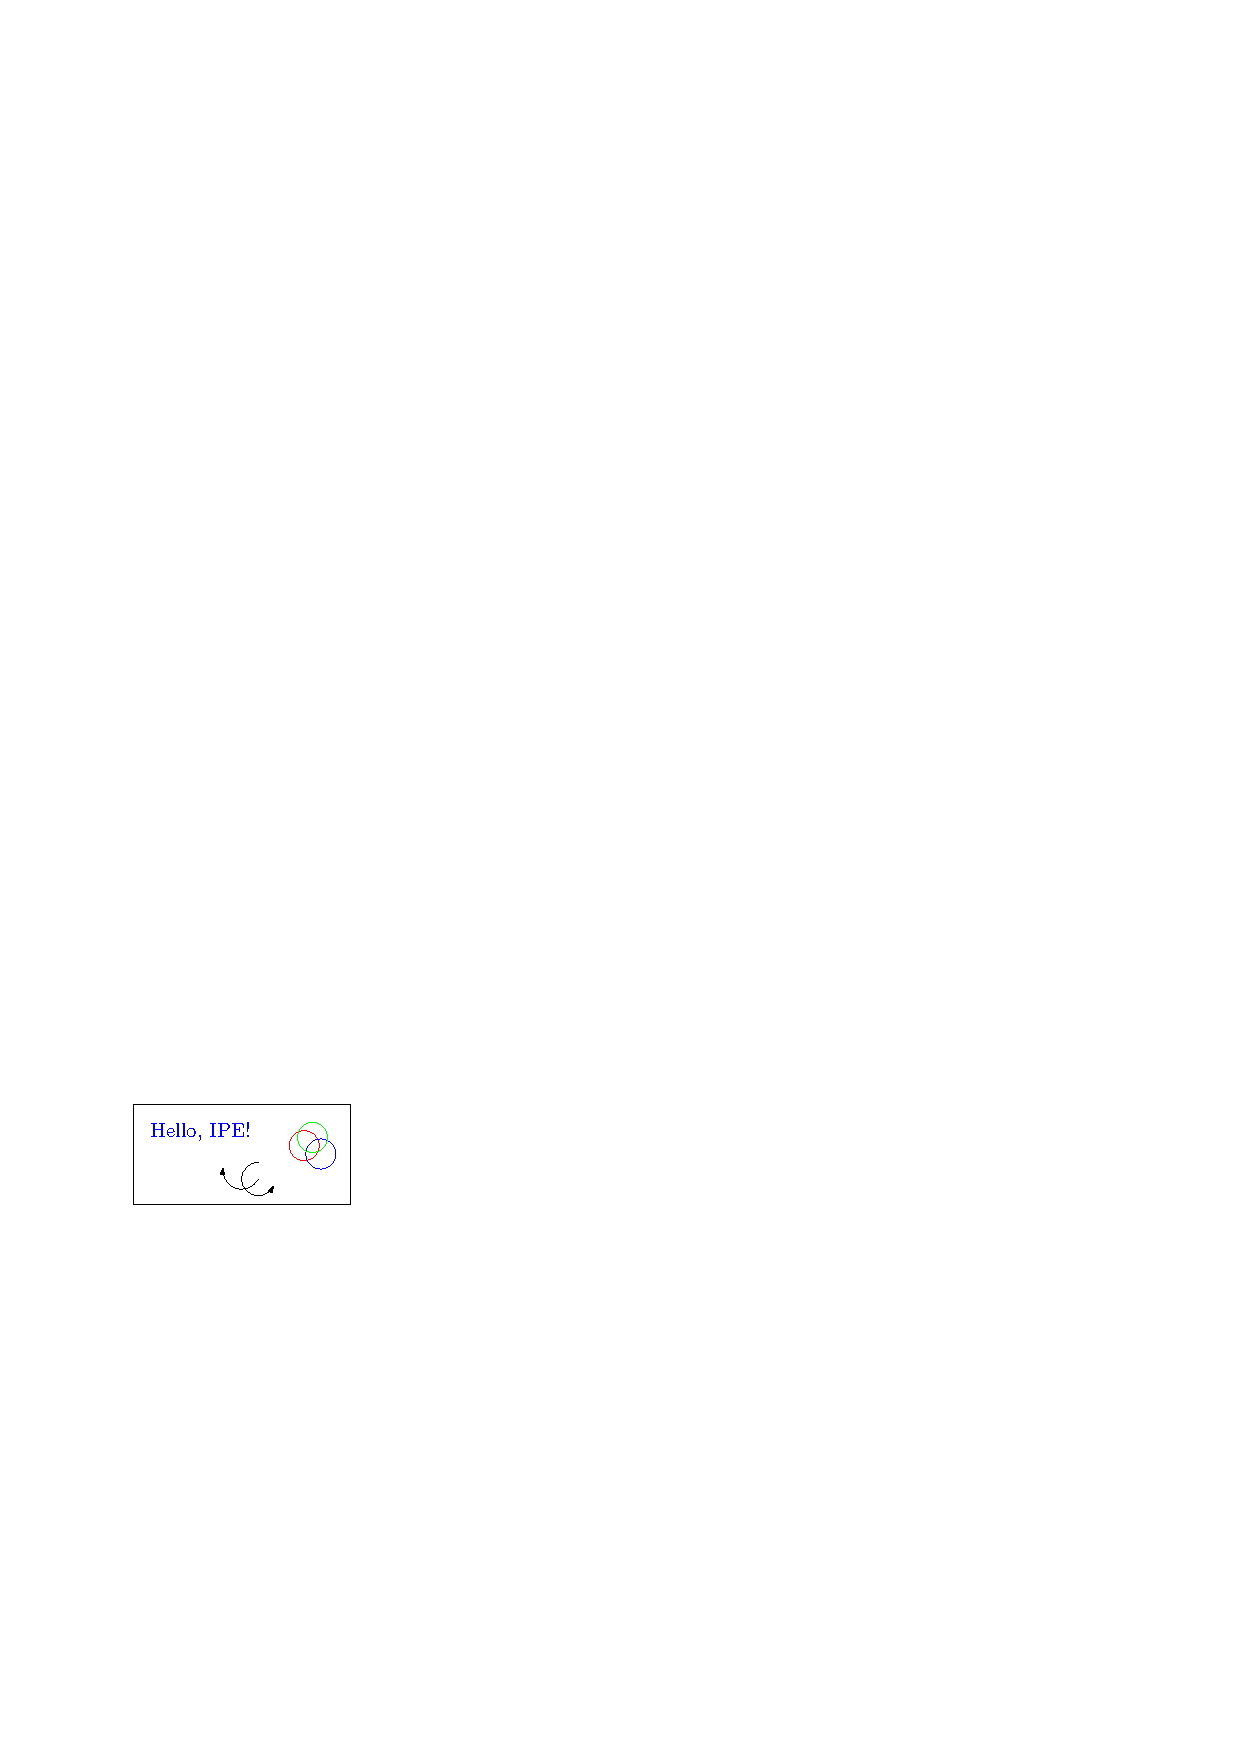
\includegraphics[width=3in]{hello}
  \caption{利用IPE制图}
  \label{fig:ipe}
\end{figure}

若子图共用一个计数器,
那么请看图~\ref{fig:big1},它包含两个小图,分别是图~\ref{fig:subfig1} 
和图~\ref{fig:subfig2}。这里推荐使用\verb|\subfloat|,{\bf 不要再用}
\verb|\subfigure|和\verb|\subtable|。
\begin{figure}[htb]
  \centering%
  \subfloat[第一个小图形]{%
    \label{fig:subfig1}
    
\includegraphics[height=2cm]{xh}}\hspace{4em}%
  \subfloat[第二个小图形。如果标题很长的话,它会自动换行,这个 caption 就是这样的例子]{%
    \label{fig:subfig2}
    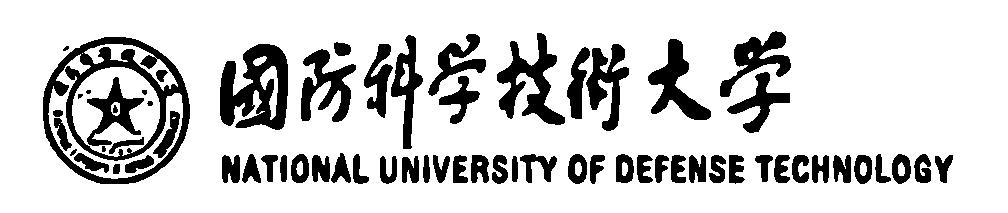
\includegraphics[height=2cm]{xhh}}
  \caption{包含子图形的大图形}
  \label{fig:big1}
\end{figure}

而下面这个例子显示并排$3\times2$的图片,见图\ref{fig:subfig:3x2}:
\begin{figure}[htb]
\centering
\subfloat[]{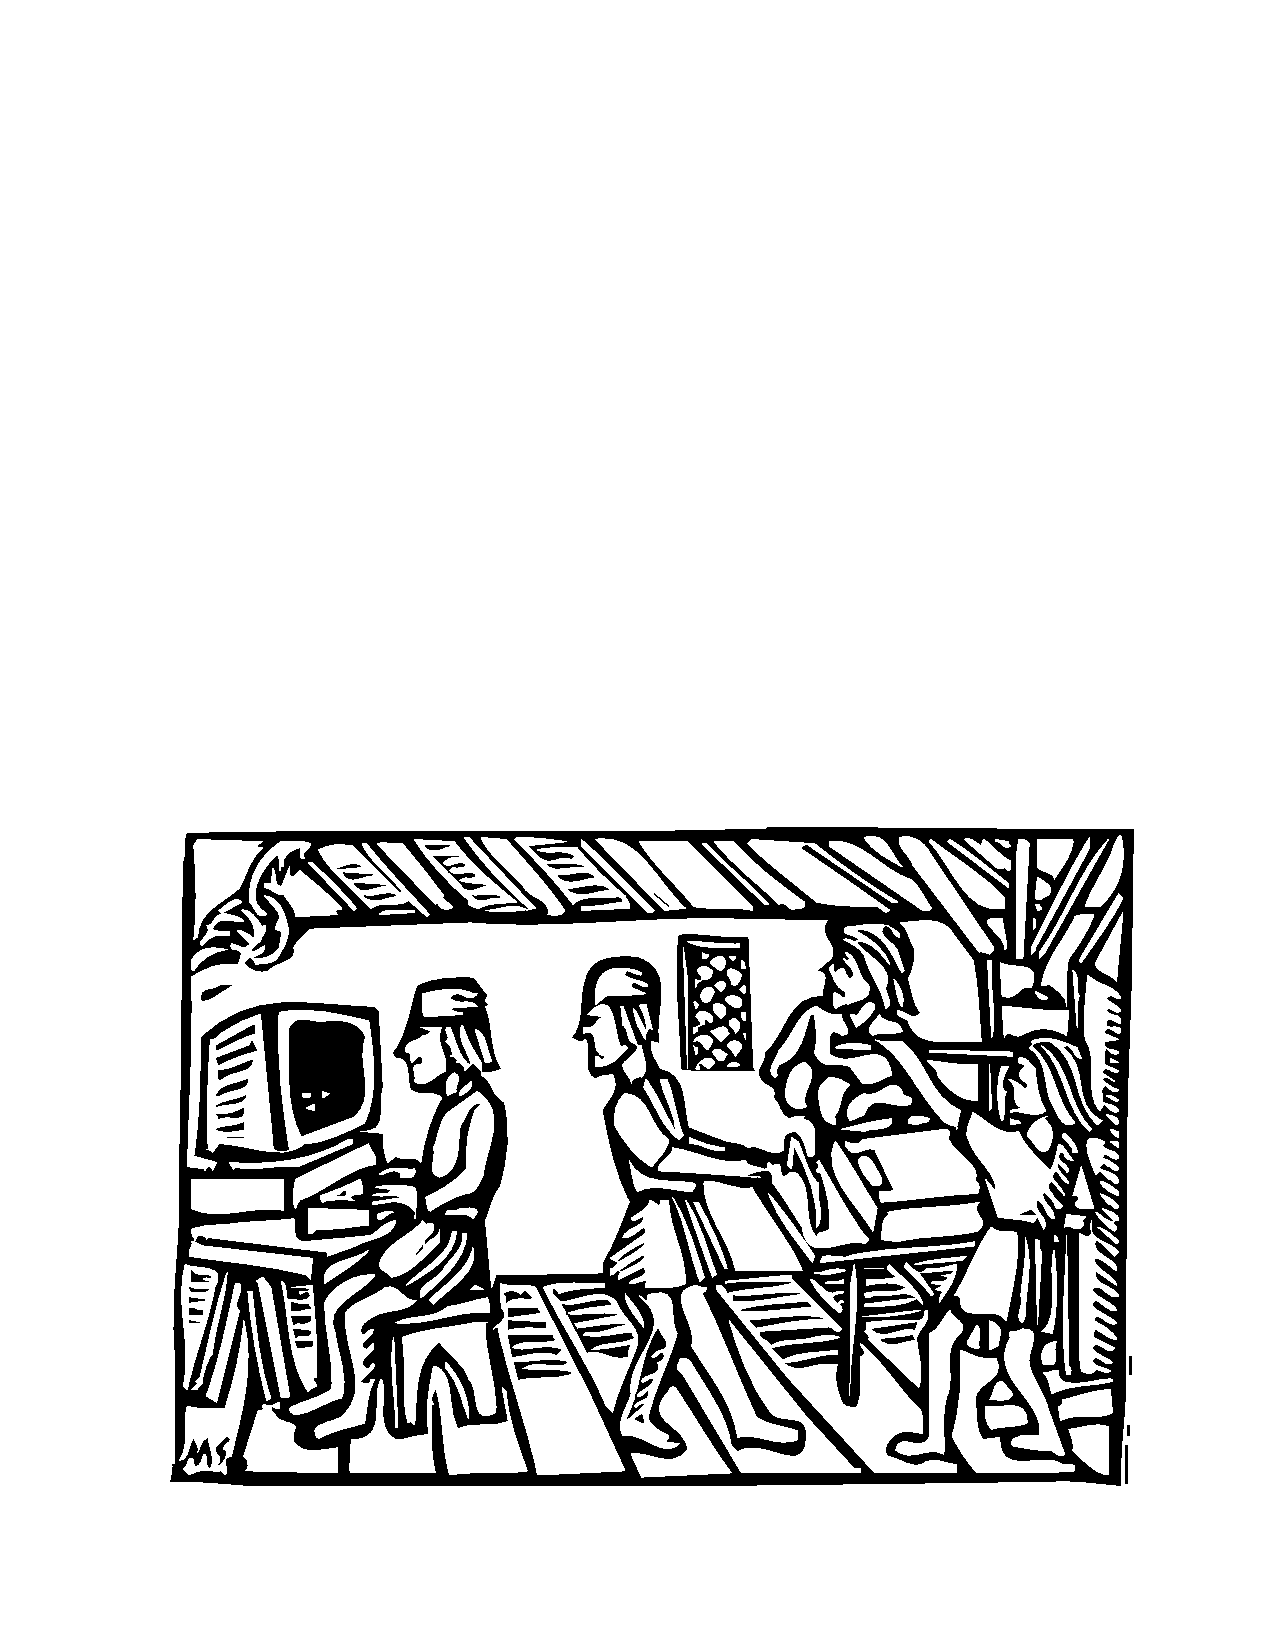
\includegraphics[width=.27\textwidth]{typography}} \qquad
\subfloat[]{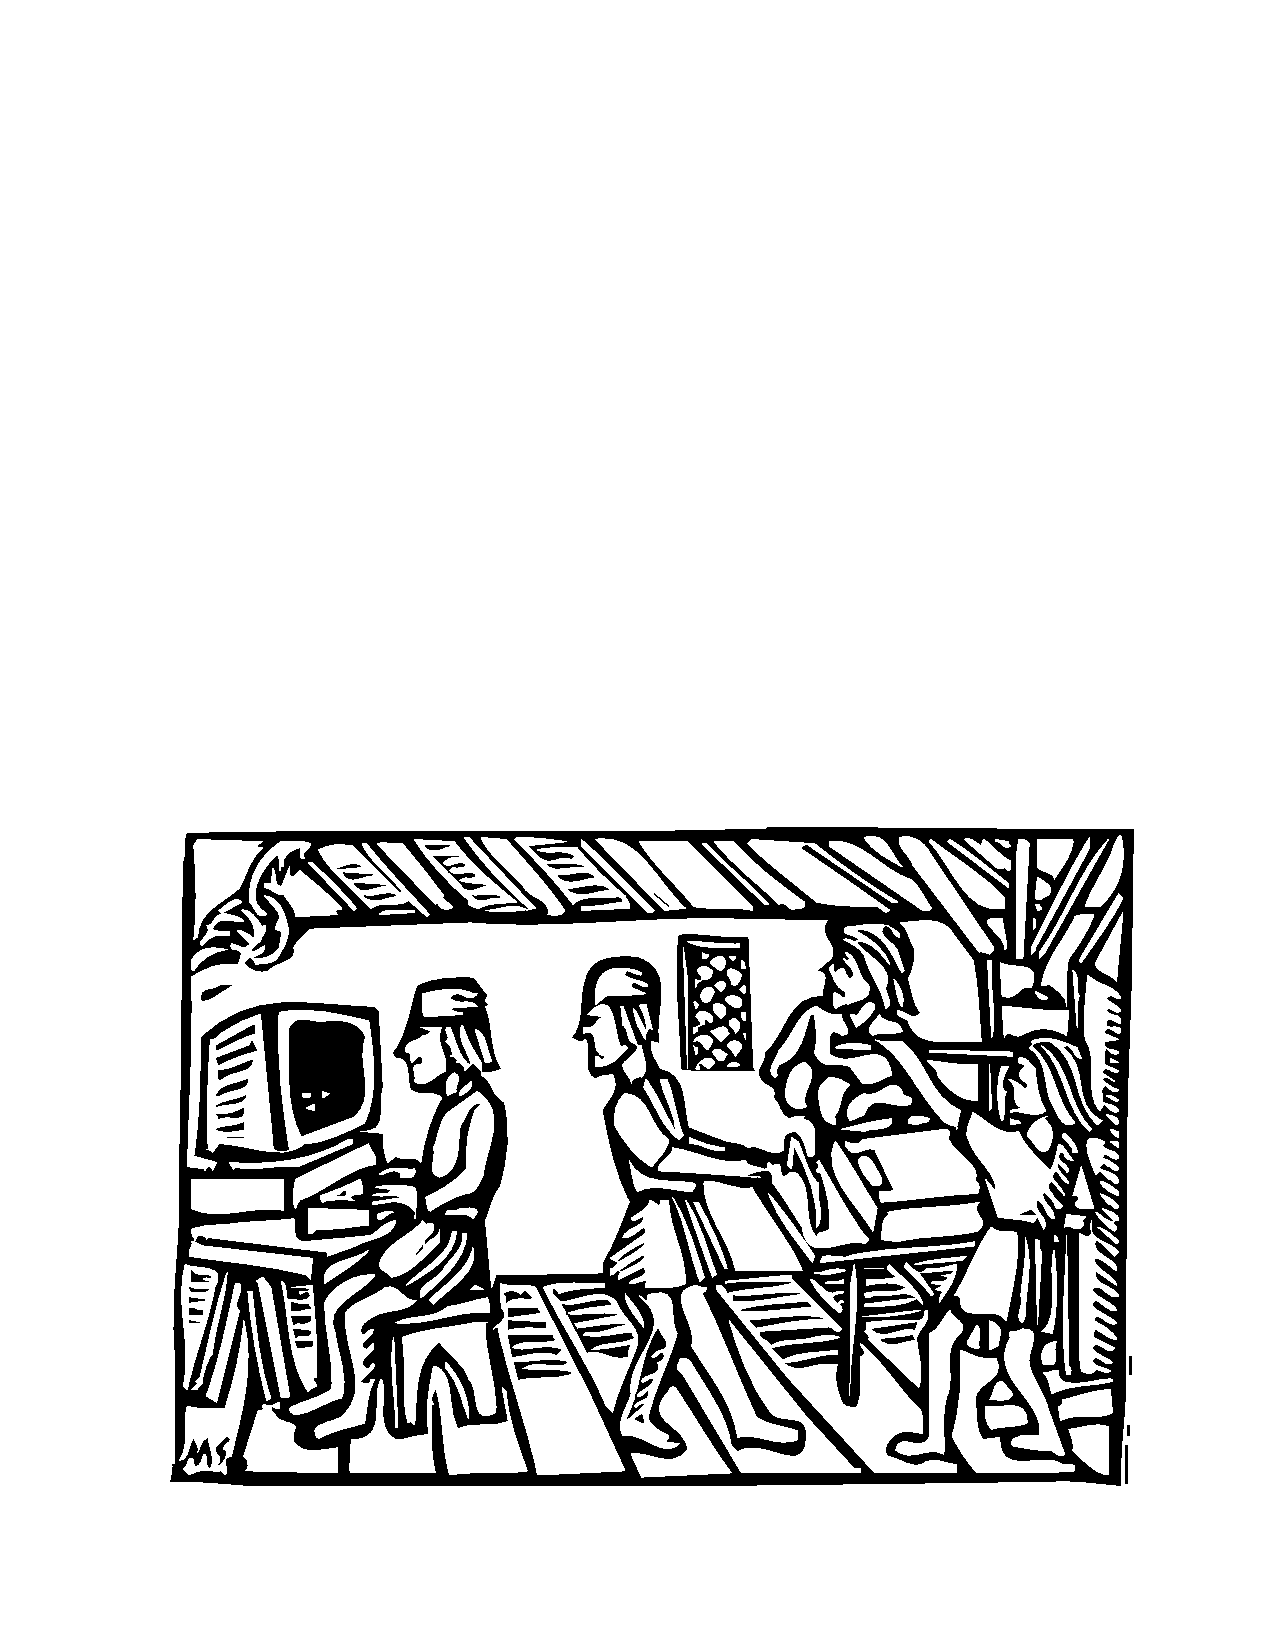
\includegraphics[width=.27\textwidth]{typography}} \qquad
\subfloat[]{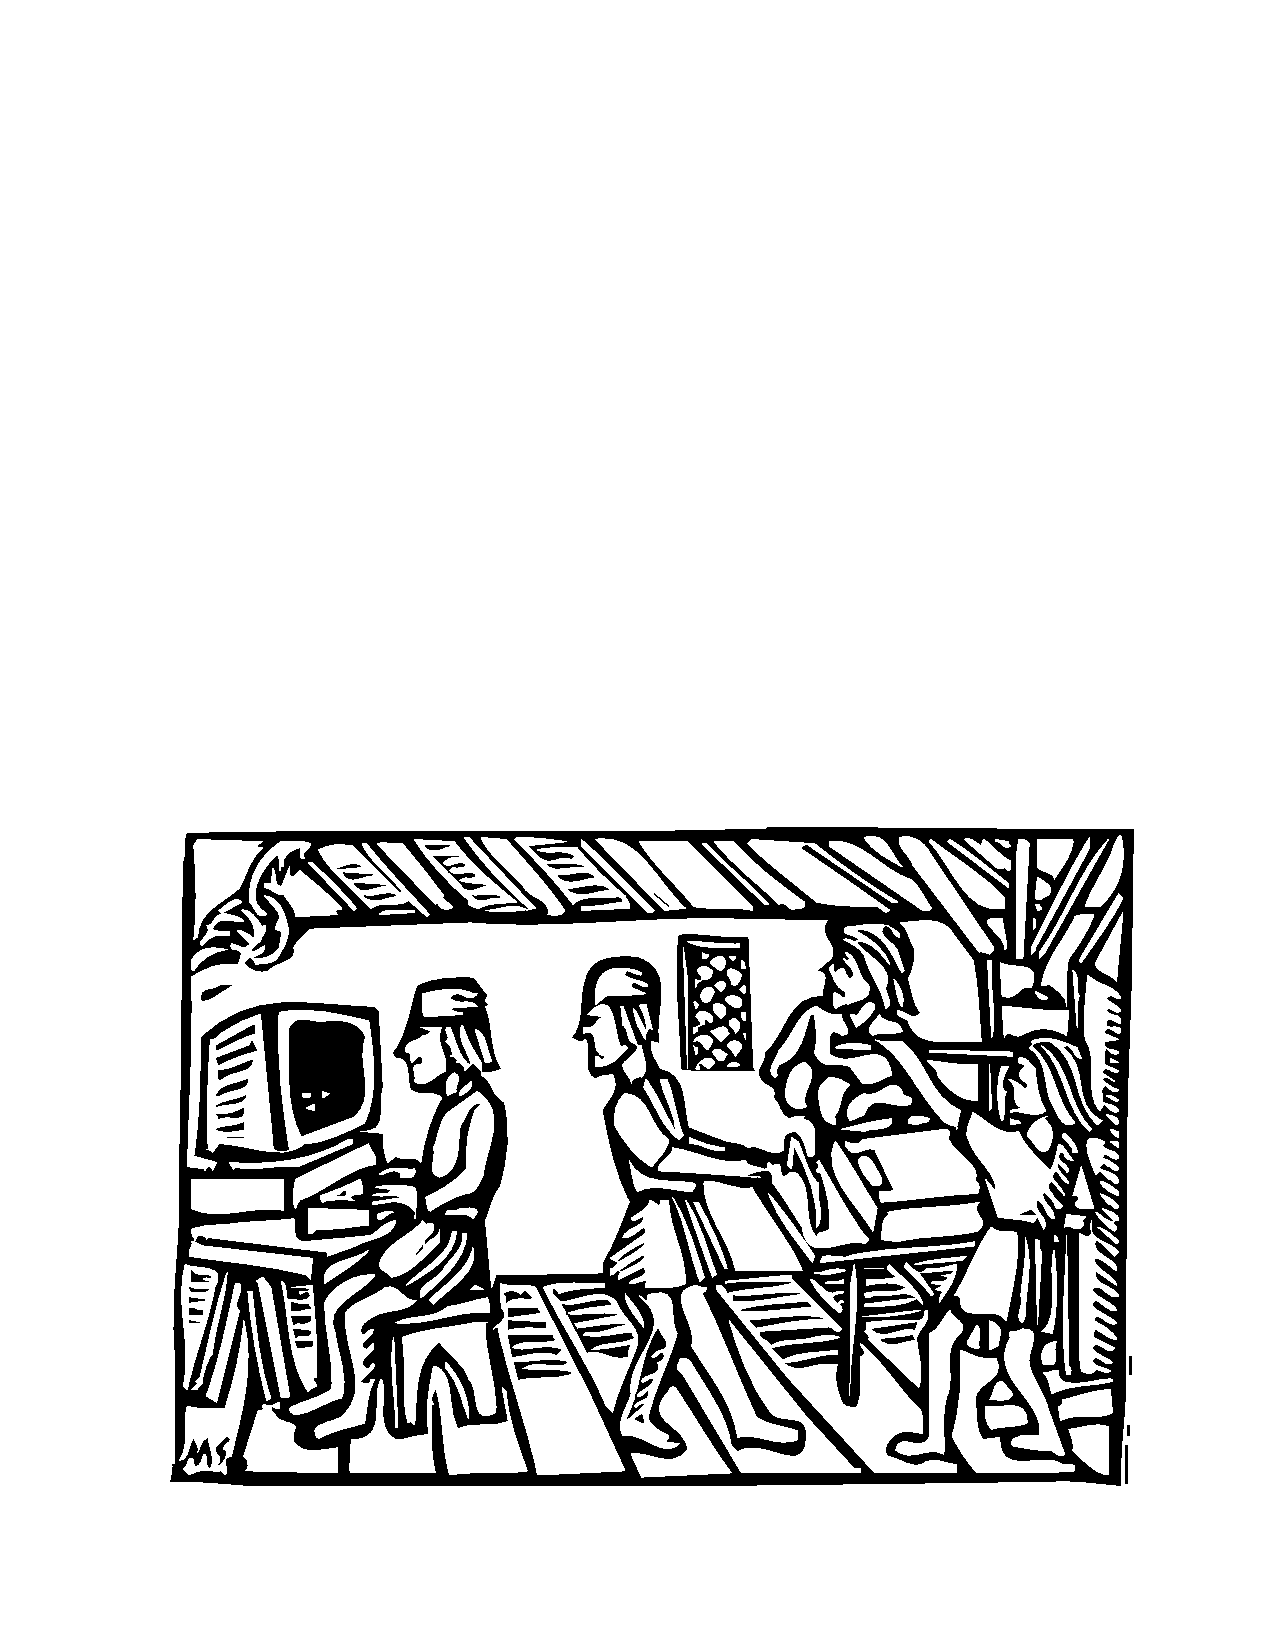
\includegraphics[width=.27\textwidth]{typography}} \qquad
\subfloat[]{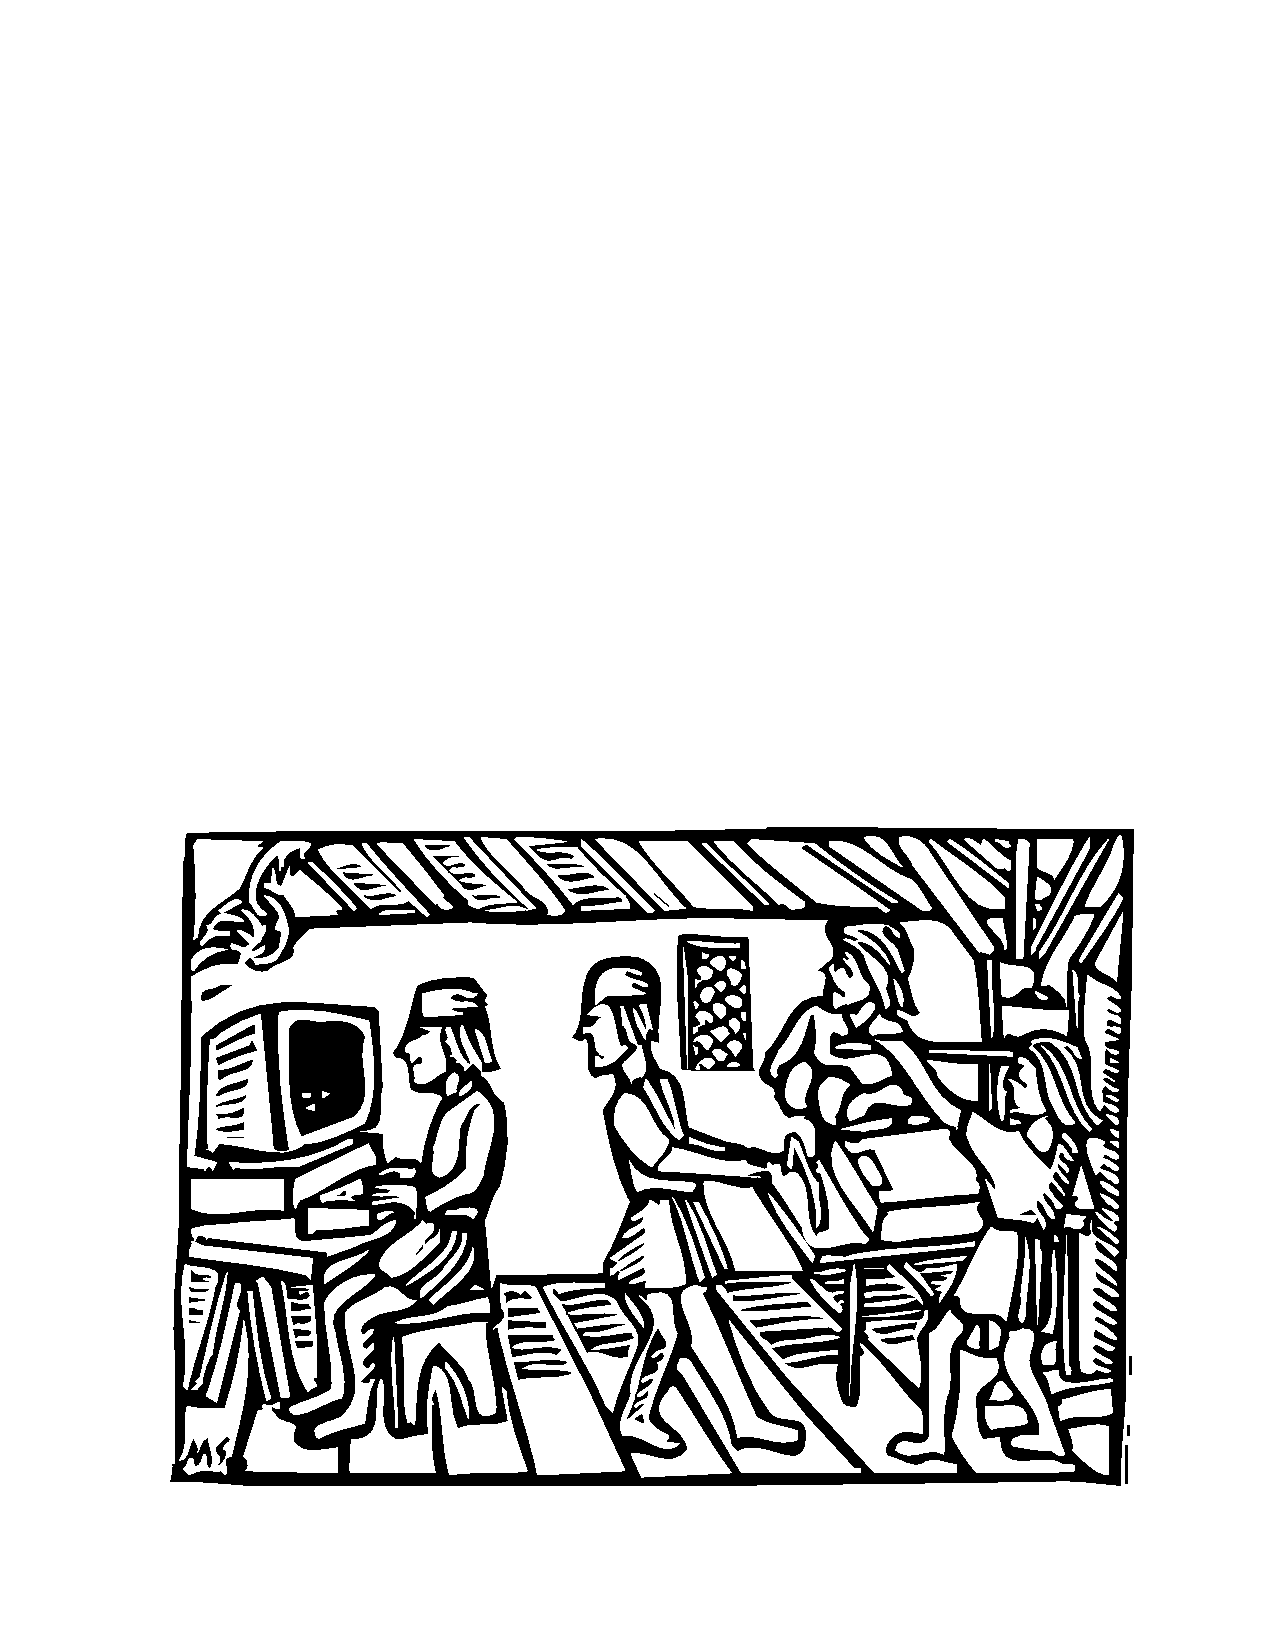
\includegraphics[width=.27\textwidth]{typography}} \qquad
\subfloat[]{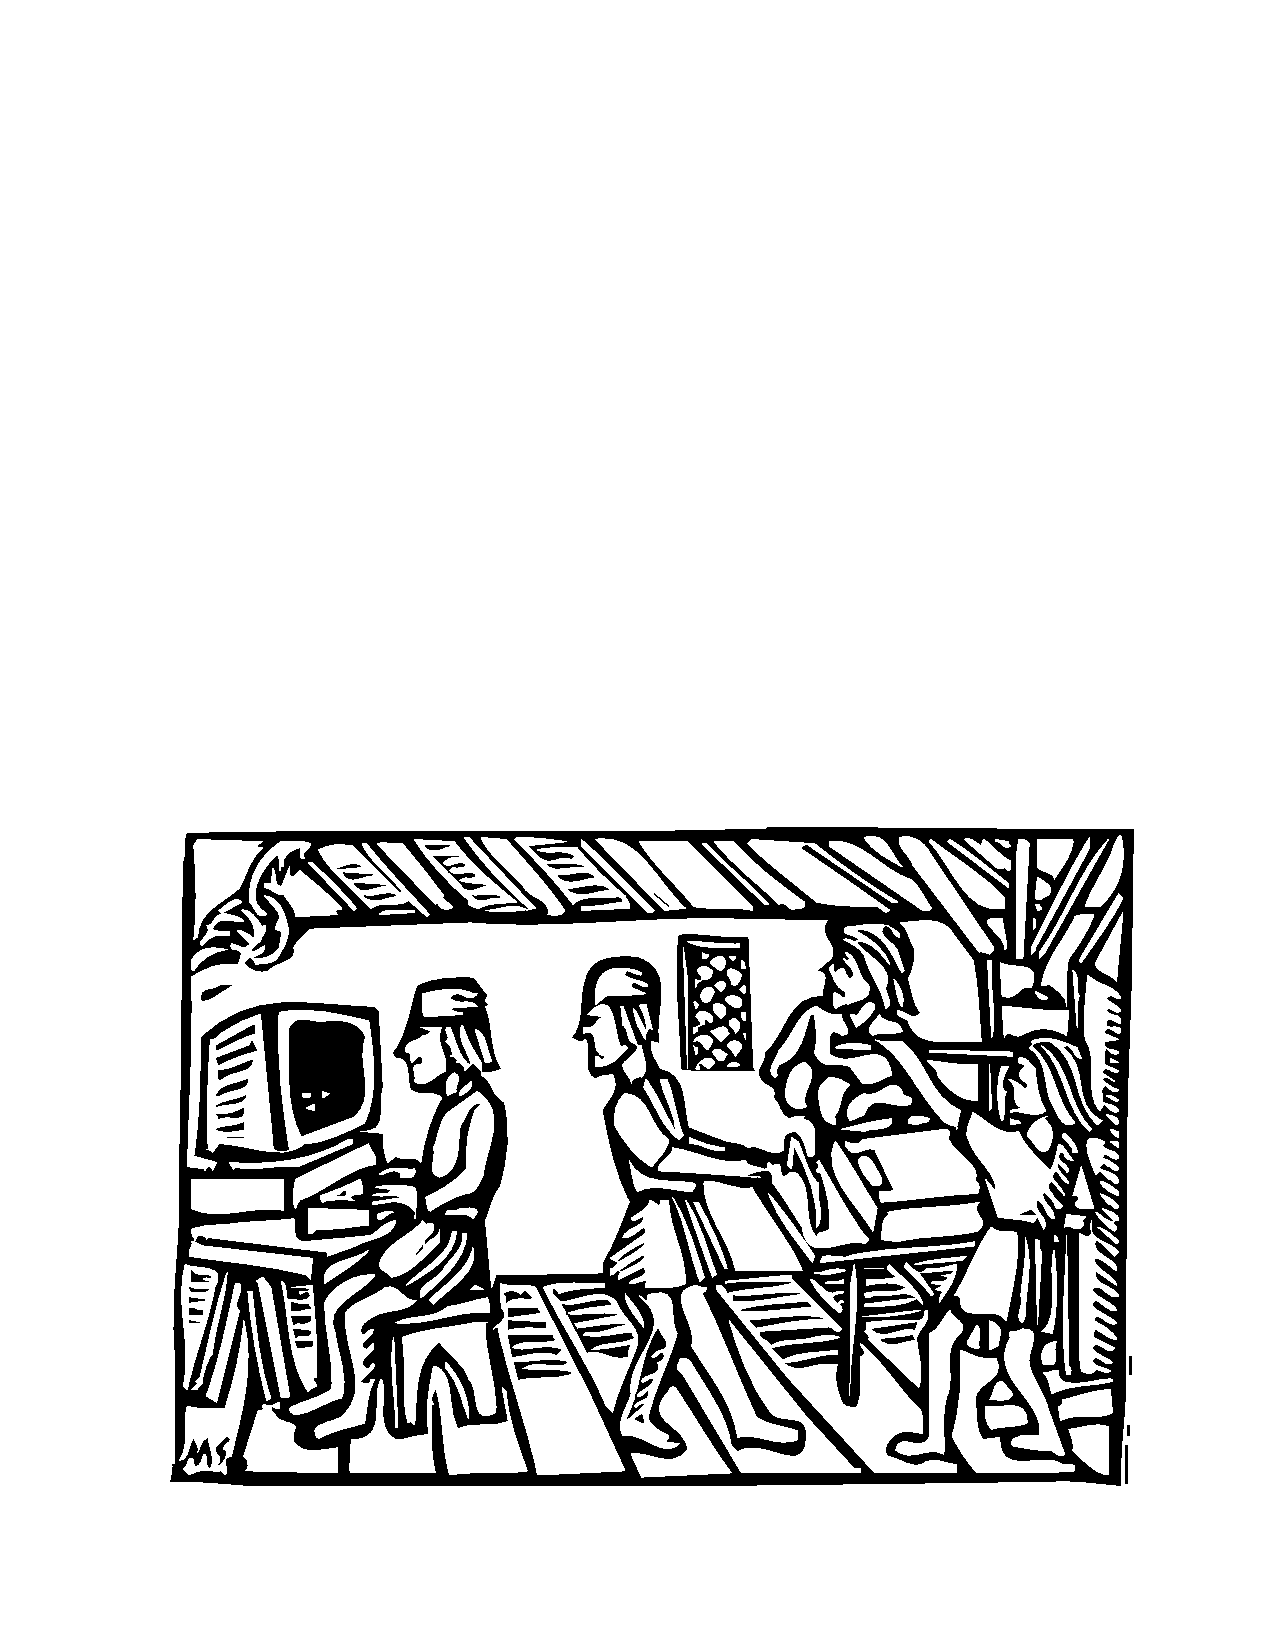
\includegraphics[width=.27\textwidth]{typography}} \qquad
\subfloat[]{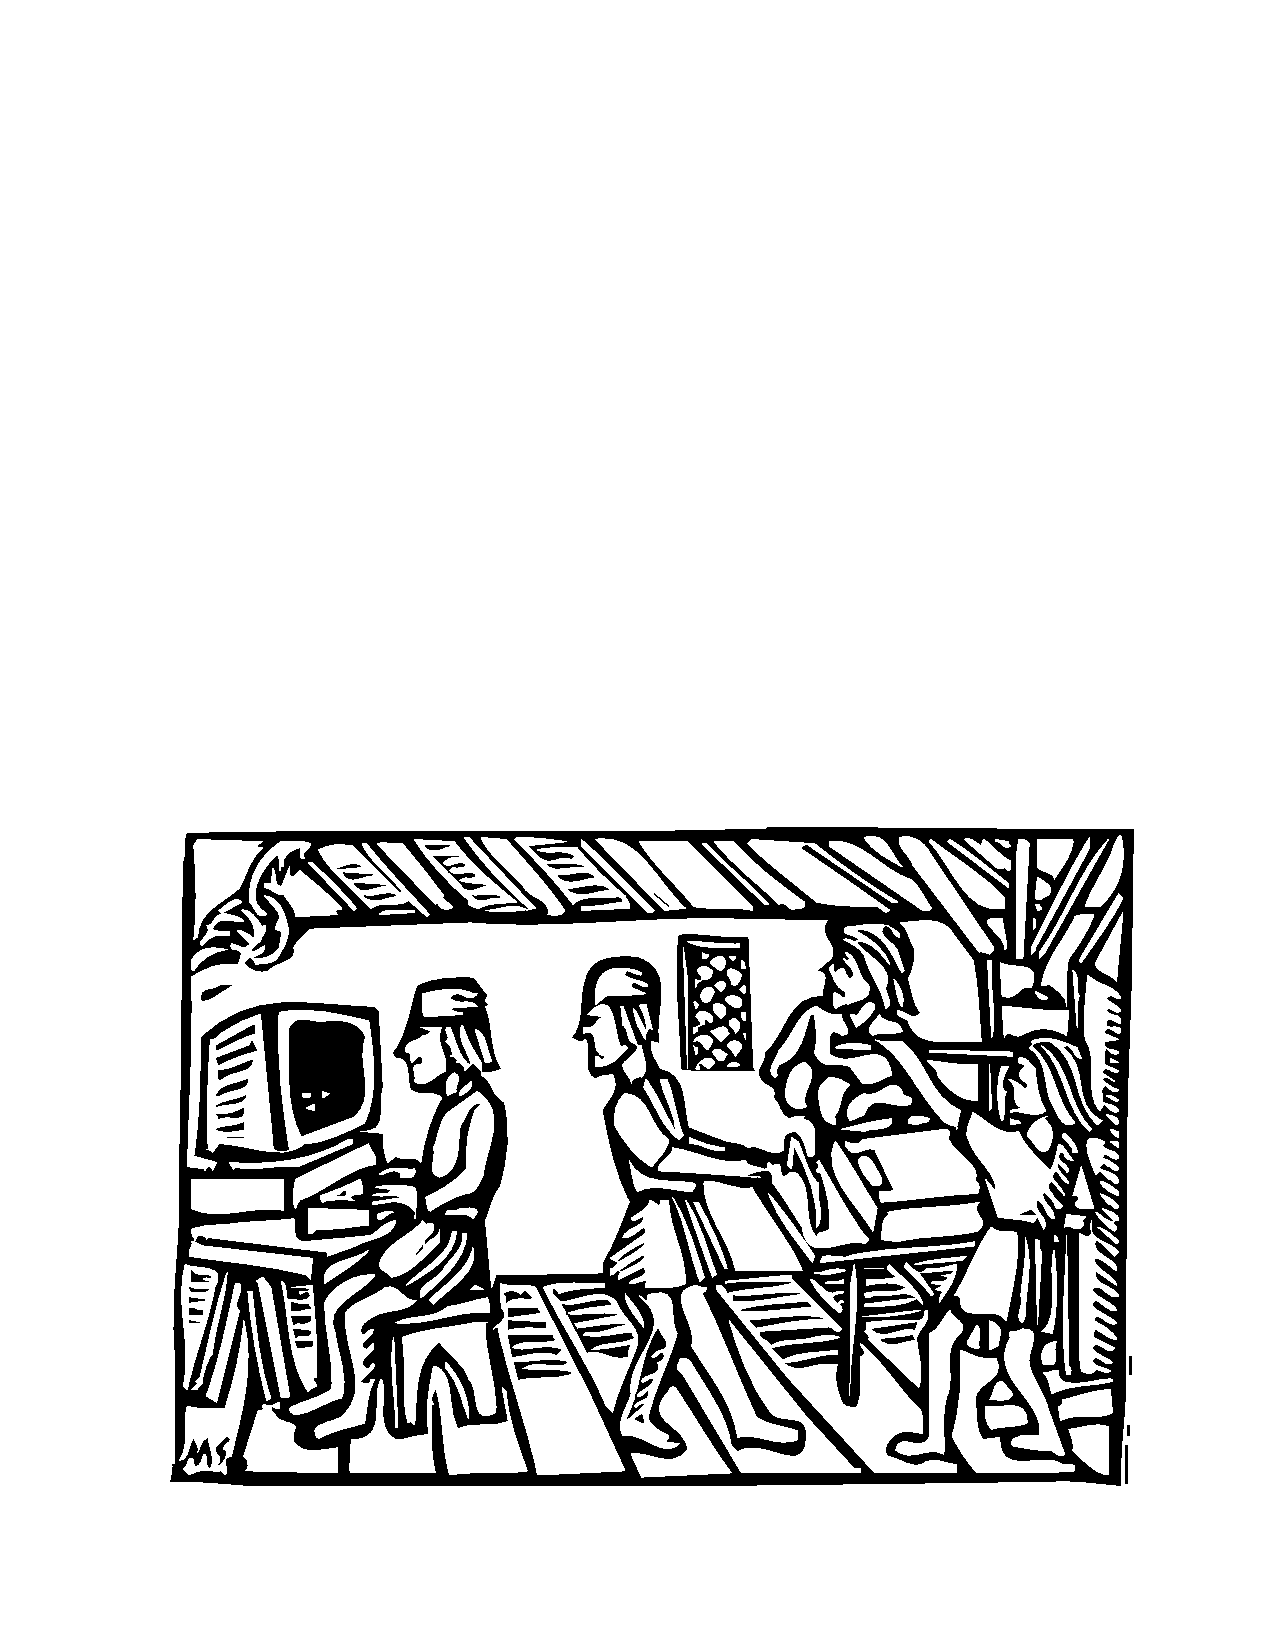
\includegraphics[width=.27\textwidth]{typography}}
\caption{并排图片}
\label{fig:subfig:3x2}
\end{figure}

要注意,图\ref{fig:subfig:3x2}例中
\texttt{qquad}相当于\verb|\hspace{2em}|,也就是2个字符的宽度,约0.08倍页宽,
图片宽度设定为0.27倍页宽是合适的;在该环境中,尽量不要手动换行,所以,不妨自己计算一下!

如果要把编号的两个图形并排,那么小页(minipage)就非常有用了,可以分别参考
图\ref{fig:parallel1}和图\ref{fig:parallel2}。其实这个例子和表格一节中并排
放置的表格一摸一样。
\begin{figure}[htb]
\begin{minipage}{0.48\textwidth}
  \centering
  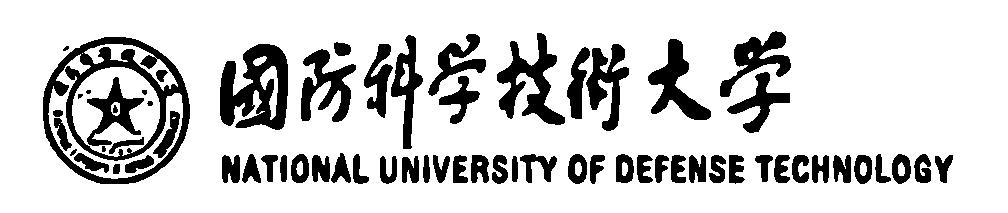
\includegraphics[height=1.2cm]{xhh}
  \caption{并排第一个图}
  \label{fig:parallel1}
\end{minipage}\hfill
\begin{minipage}{0.48\textwidth}
  \centering
  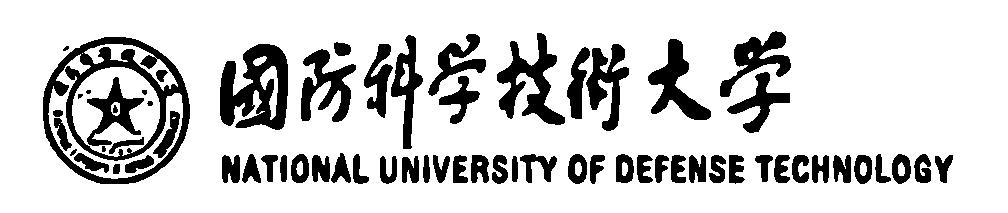
\includegraphics[height=1.2cm]{xhh}
  \caption{并排第二个图}
  \label{fig:parallel2}
\end{minipage}
\end{figure}

图形就说这么多,因为大家在写论文是遇到的最大问题不是怎么把图插进去,
而是怎样做出专业的、诡异的、震撼的图片来,记得在这时参考前面推荐的那
些工具吧,当然必不可少的是Matlab了,至于如何加入中文标注、支持中文等等
可以上网去查,但这里{\kai 推荐一点},用好export命令,使得插入图片时尽可能的不要
缩放,保证图文的一致性。

\section{公式定理}
\label{sec:equation}
贝叶斯公式如式~(\ref{equ:chap1:bayes}),其中$p(y|\mathbf{x})$为后验;
$p(\mathbf{x})$为先验;分母$p(\mathbf{x})$ 为归一化因子,这是
实际应用中十分恐怖的一个积分式。
\begin{equation}
\label{equ:chap1:bayes}
p(y|\mathbf{x}) = \frac{p(\mathbf{x},y)}{p(\mathbf{x})}=
\frac{p(\mathbf{x}|y)p(y)}{p(\mathbf{x})} 
\end{equation}

论文里面公式越多,\TeX{} 就越 happy。再看一个 \textsf{amsmath} 的例子:
\newcommand{\envert}[1]{\left\lvert#1\right\rvert} 
\begin{equation}\label{detK2}
\det\mathbf{K}(t=1,t_1,\dots,t_n)=\sum_{I\in\mathbf{n}}(-1)^{\envert{I}}
\prod_{i\in I}t_i\prod_{j\in I}(D_j+\lambda_jt_j)\det\mathbf{A}
^{(\lambda)}(\overline{I}|\overline{I})=0.
\end{equation} 

大家在写公式的时候一定要好好看\textsf{amsmath}的文档,并参考模板中的用法:
\begin{multline*}%\tag{[b]} % 这个出现在索引中的
\int_a^b\biggl\{\int_a^b[f(x)^2g(y)^2+f(y)^2g(x)^2]
 -2f(x)g(x)f(y)g(y)\,dx\biggr\}\,dy \\
 =\int_a^b\biggl\{g(y)^2\int_a^bf^2+f(y)^2
  \int_a^b g^2-2f(y)g(y)\int_a^b fg\biggr\}\,dy
\end{multline*}

再看\ref{equ:split}:
\begin{equation}\label{equ:split}
\begin{split}
C(z) &= [z^n] \biggl[\frac{e^{3/4}}{\sqrt{1-z}} +
e^{-3/4}(1-z)^{1/2} + \frac{e^{-3/4}}{4}(1-z)^{3/2}
+ O\Bigl( (1-z)^{5/2}\Bigr)\biggr] \\
&= \frac{e^{-3/4}}{\sqrt{\pi n}} - \frac{5e^{-3/4}}{8\sqrt{\pi
n^3}} + \frac{e^{-3/4}}{128 \sqrt{\pi n^5}} +
O\biggl(\frac{1}{\sqrt{\pi
n^7}}\biggr)
\end{split}
\end{equation}

当然了,数学中必不可少的是定理和证明:
\begin{theorem}
  \label{chapTSthm:rayleigh solution}
  假定 $X$ 的二阶矩存在:
  \begin{equation}
         O_R(\mathbf{x},F)=\sqrt{\frac{\mathbf{u}_1^T\mathbf{A}\mathbf{u}_1} {\mathbf{u}_1^T\mathbf{B}\mathbf{u}_1}}=\sqrt{\lambda_1},
  \end{equation}
  其中 $\mathbf{A}$ 等于 $(\mathbf{x}-EX)(\mathbf{x}-EX)^T$,$\mathbf{B}$ 表示协方差阵 $E(X-EX)(X-EX)^T$,$\lambda_1$
$\mathbf{u}_1$是$\lambda_1$对应的特征向量,
\end{theorem}

对于希腊符号使用\verb|mathbf|命令可能有些问题,所以建议对符号
用\verb|bm|加粗,记得用\verb|\up<greek>|切换正体符号,下面看几个例子:
\verb|\gamma|斜体代表变量$\gamma$,\verb|\bm{\upgamma}|正体代表向量$\bm{\upgamma}$,
。\verb|\Gamma|正体代表操作符号$\Gamma$,
\verb|\bm{\Gamma}|正体粗体代表矩阵形式$\bm{\Gamma}$,
\verb|\varGamma|斜体代表变量$\varGamma$。另外对于大小写斜体的加粗可以见$\bm{\gamma}$和$\bm{\varGamma}$,
但是这两种科技论文中很少出现,这里只做测试。
非符号普通向量就用\verb|\mathbf|吧:$\mathbf{x}_k,\mathbf{X}_k$。
完整测试如下$\omega,\bm{\omega},\upomega,\bm{\upomega},\Omega,\bm{\Omega},\varOmega,\bm{\varOmega}$。

\begin{proof}
上述优化问题显然是一个Rayleigh商问题。我们有
  \begin{align}
     O_R(\mathbf{x},F)=\sqrt{\frac{\mathbf{u}_1^T\mathbf{A}\mathbf{u}_1} {\mathbf{u}_1^T\mathbf{B}\mathbf{u}_1}}=\sqrt{\lambda_1},
 \end{align}
 其中 $\lambda_1$ 下列广义特征值问题的最大特征值:
$$
\mathbf{A}\mathbf{z}=\lambda\mathbf{B}\mathbf{z}, \mathbf{z}\neq 0.
$$
 $\mathbf{u}_1$ 是 $\lambda_1$对应的特征向量。结论成立。
\end{proof}

下面来看看算法环境的定义和使用。
我们知道,故障诊断的最终目的,是将故障定位到部件,而由于信号--部件依赖矩阵的存在,因此,实质性的工作是找出由故障部件发出异常信号,
不妨称为源异常信号,而如前所述,源异常信号与异常信号依赖矩阵$\mathbf{S_a}$的全零列是存在一一对应的关系的。因此,我们只要获得了$\mathbf{S_a}$的全零列的相关信息,
也就获得了源异常信号的信息,从而能进一步找到故障源。
通过以上分析,我们构造算法\ref{alg53},用于实现非回路故障诊断。
\begin{algorithm}[htbp]
  \caption{非回路故障诊断算法}
  \label{alg53}
  \begin{algorithmic}[1]
    \REQUIRE 信号--部件依赖矩阵$\mathbf{A}$,信号依赖矩阵$\mathbf{S}$,信号状态向量$\alpha$
    \ENSURE 部件状态向量$\gamma$
    \STATE $\mathbf{P}\leftarrow\left(<\alpha>\right)$
    \STATE $\mathbf{S_{a}}\leftarrow\mathbf{P^T}\mathbf{S}\mathbf{P}$
    \FOR{$i=1$ to $S_a$的阶数$m$}
    \STATE $s_i\leftarrow s_i$的第$i$个行向量
    \ENDFOR
    \STATE $\beta_a\leftarrow\lnot \left(s_1\lor s_2\lor \cdots\lor s_m\right)^T$
    \STATE $\beta\leftarrow\mathbf{P}\beta_a$
    \STATE $\gamma\leftarrow\mathbf{A}\beta$
  \end{algorithmic}
\end{algorithm}

第一类故障回路推理与非回路故障推理是算法基本相同,稍微不同的是$\beta_a$的计算。因为第一类故障回路中的信号全部可能是源异常信号,因此我们不必计算
$\beta_a=\lnot \left(\left[s_1\lor s_2\lor \cdots\lor s_m\right]^T\right)$,而直接取$\beta_a=\underbrace{\left[\begin{array}{cccc}1&1&\cdots&1\end{array}\right]^T}_m$,将$\beta_a$代入
算法\ref{alg53},有
\[\beta=\mathbf{P}\beta_a=\mathbf{P}\underbrace{\left[\begin{array}{cccc}1&1&\cdots&1\end{array}\right]^T}_m=\alpha\]
因此一类故障回路的推理算法变得相当简单,例如算法\ref{alg54}
\begin{algorithm}[htbp]
  \caption{第一类故障回路诊断算法}
  \label{alg54}
  \begin{algorithmic}[1]
    \REQUIRE 信号--部件依赖矩阵$\mathbf{A}$,信号状态向量$\alpha$
    \ENSURE 部件状态向量$\gamma$
    \STATE $\gamma\leftarrow\mathbf{A}\alpha$
  \end{algorithmic}
\end{algorithm}

\section{参考文献}
\label{sec:bib}
当然参考文献可以直接写 bibitem,虽然费点功夫,但是好控制,各种格式可以自己随意改
写,在nudtpaper里面,建议使用JabRef编辑和管理文献,再结合\verb|bstutf8.bst|,
对中文的支持非常不错,格式也很规范。

本模板推荐使用 BIB\TeX,样式文件为 bstutf8.bst,符合学校的参考文献格式(如专利
等引用未加详细测试)。看看这个例子,关于书的\upcite{tex, companion},
还有这些\upcite{Krasnogor2004e, clzs, zjsw},关于杂志的\upcite{ELIDRISSI94,
  MELLINGER96, SHELL02},硕士论文\upcite{zhubajie, metamori2004},博士论文
\upcite{shaheshang, FistSystem01},标准文件\upcite{IEEE-1363},会议论文\upcite{DPMG,kocher99},%
技术报告\upcite{NPB2}。中文参考文献\upcite{cnarticle}\textsf{特别注意},需要在\verb|bibitem|中
增加\verb|language|域并设为\verb|zh|,英文此项可不填,之后由\verb|bstutf8|统一处理
(具体就是决定一些文献在中英文不同环境下的显示格式,如等、etc)。
若使用\verb|JabRef|,则你可按下面步骤来设置:
选择\textsf{Options}$\rightarrow$\textsf{Set Up General Fields},
在\verb|General:|后加入\verb|language|就可以了。

有时候不想要上标,那么可以这样 \cite{shaheshang},这个非常重要。

\section{代码高亮}
有些时候我们需要在论文中引入一段代码,用来衬托正文的内容,或者体现关键思路的实现。
在模板中,统一使用\texttt{listings}宏包,并且设置了基本的内容格式,并建议用户只
使用三个接口,分别控制:编程语言,行号以及边框。简洁达意即可,下面分别举例说明。

首先是设定语言,来一个C的,使用的是默认设置:
\begin{lstlisting}[language=C]
void sort(int arr[], int beg, int end)
{
  if (end > beg + 1)
  {
    int piv = arr[beg], l = beg + 1, r = end;
    while (l < r)
    {
      if (arr[l] <= piv)
        l++;
      else
        swap(&arr[l], &arr[--r]);
    }
    swap(&arr[--l], &arr[beg]);
    sort(arr, beg, l);
    sort(arr, r, end);
  }
}
\end{lstlisting}

当我们需要高亮Java代码,不需要行号,不需要边框时,可以:
\begin{lstlisting}[language=Java,numbers=none,frame=none]
// A program to display the message
// "Hello World!" on standard output

public class HelloWorld {
 
   public static void main(String[] args) {
      System.out.println("Hello World!");
   }
      
}   // end of class HelloWorld
\end{lstlisting}

细心的用户可能发现,行号被放在了正文框之外,事实上这样是比较美观的,
如果有些用户希望在正文框架之内布置所有内容,可以:
\begin{lstlisting}[language=perl,xleftmargin=2em,framexleftmargin=1.5em]
#!/usr/bin/perl
print "Hello, world!\n";
\end{lstlisting}

好了,就这么多,\texttt{listings}宏包的功能很强大也很复杂,如果需要自己定制,
可以查看其手册,耐心阅读总会找到答案。
\textbf{注意:} 当前代码环境中文注释的处理还不是很完善,对于注释请妥善处理。
在本模板中,推荐算法环境或者去掉中文的listings代码环境。
如果需要包含中文注释,不要求代码高亮,
就用\texttt{code}环境,这个环境是Verbatim的定制版,简单有效,
调用的是fancyvbr宏包,用户可在mynudt.sty中修改它的外观等等。
这里我们还可以给代码加上标签。
\begin{code}[label=hello.c]
public class HelloWorld {
   public static void main(String[] args) {
      System.out.println("Hello World!");
   }
}   // 世界,你好!
\end{code}

\section{符号列表}

{\hei 前面的话:}{\kai\color{blue} 
2.2版本后默认使用nomencl环境,如果你还是希望使用传统的\verb|definition.tex|,那么只需注释掉
顶层文件中的nomenclature即可。}

符号列表使用的是\verb|nomencl|包,自己简单定制了下,使用方法分为四步:
\begin{compactenum}
\item 将\verb|\makenomenclature|语句放在正文前,即\verb|\begin{document}|前面;
\item 将\verb|\printnomenclature|放在论文中,我在例子中将符号列表放在了英文摘要的
后面,正文第一章的前面,当然,你可以根据自己的需要或者教研室的规范放置在合理的位置上,
为了页面引用的正确,在这句话前面放上\verb|\cleardoublepage|;
\item 使用\verb|\nomenclature|命令在论文的各个位置上添加符号定义,语法后面会讲到;
\item 编译。编译需要首先运行一遍xelatex,之后运行
\begin{code}
makeindex -s nomencl.ist -o thesis.nls thesis.nlo
\end{code}
\end{compactenum}

你可以把这句编译命令放在\verb|makepdf.bat|中第一个\verb|xelatex thesis|下面。然后
双击\verb|makepdf.bat|就可以了,论文模板中已经为你添加上了,如果你强烈不想使用
nomencl环境,只要把它注释掉(前面加\verb|rem|)就可以。
另外,由于我使用的是VIM来编辑\TeX{}代码,具体到每个编辑器(诸如WinEDT,TeXWorks等)
如何设定该命令的快捷按钮,诸位可以搜索网上的教程。

下面简单说明下\verb|\nomenclature|命令,语法为。这里插入一些随机的文字,希望
对你在阅读帮助中的思维没有什么不良的影响。
\begin{code}
\nomenclature[<prefix>]{<symbol>}{<desc>}{<null>}
\end{code}
\verb|nomencl|模板的默认排序方法可能(大多都)不满足要求,
论文模板里,我们通过设定\verb|<prefix>|来实现符号列表的排序。
它分为两部分,比如如\verb|[Aa]|,第一个字母的含义是:
\begin{compactitem}
\item[`A'] 符号归为拉丁字母
\item[`G'] 希腊字母
\item[`X'] 上标
\item[`Z'] 下标
\end{compactitem}
每个标识后边的字幕\verb|a-z|作为当前符号组内的排列顺序,比如$\beta$就可以写成
\verb|[Gb]|,诸如此类。当然你一定注意到了,这个排序分组的设定只是为了记忆
方便,并不是强制的,因此你可以有自己的方案,比如Z是Greek,
R是Roman什么的,只要统一就好,只需记住,组间排列是按字母顺序排的。

注意符号表分四列,前三列的含义与命令中相同,
最后一列是符号定义时所在的页码。效果看例子,对于下式:
\begin{equation}\label{eq:heatflux}
   \dot{Q} = k \cdot A \cdot \Delta T
\end{equation}%
\nomenclature[Aq]{$\dot{Q}$}{heat flux}{}%
\nomenclature[Ak]{$k$}{overall heat transfer coefficient,式\eqref{eq:ohtc}}{}%
\nomenclature[Aa]{$A$}{area}{}%
\nomenclature[Al]{$L$}{length}{}%
\nomenclature[At]{$T$}{temperature}{}%
\nomenclature[At]{$\Delta T$}{temperature difference}{}%
\nomenclature[Gr]{$\gamma$}{中文测试, 以及一句很长的物理意义,很有可能超过当前栏的宽度,主要目的是看一看会不会出现某些异常情况。}{}%

或者:
\begin{equation}\label{eq:ohtc}
    \frac{1}{k} = \left[\frac{1}{\alpha _{\mathrm{i}}\,r_{\mathrm{i}}} +
    \sum^n_{j=1}\frac{1}{\lambda _j}\,
    \ln \frac{r_{\mathrm{a},j}}{r_{\mathrm{i},j}} +
    \frac{1}{\alpha _{\mathrm{a}}\,
    r_{\mathrm{a}}}\right] \cdot r_{\mathrm{reference}}
\end{equation}%
\nomenclature[Ga]{$\alpha$}{convection heat transfer coefficient}{}%
\nomenclature[Zi]{i}{in}{}%
\nomenclature[Gl]{$\lambda$}{thermal conductivity}{}%
\nomenclature[Za]{a}{out}{}%
\nomenclature[Zn]{$n$}{number of walls}{}%
\nomenclature[Zj]{$j$}{running parameter}{}%

{\hei 注意事项:}{\kai 模板中定制的nomencl格式在mynudt.sty中,默认是三栏的,分别是:
``符号'',``定义'',``首次出现页码'',
注意这里的符号列表都没有单位,如果你需要额外的栏输入单位(呵呵,聪明的读者可能看出来
了,\verb|nomenclature|命令最后一个是空的,就是用来让你赋予她各种意义的)。
此时就需要你有一点点动手能力了(其实只要会修改表格就行),
方法很简单,比如需要添加``国际单位制''这一栏,则
\begin{compactenum}
\item 论文中\verb|\nomenclature|命令的第三个参数就让他代表单位,也可留空;
\item 将\verb|mynudt.sty|中longtable的表头添加``国际单位制''几个字,
你也可以取其他的名字,放在那个{\kai 应该出现的}位置上;
\item 由于增加了5个字,就把前面栏的宽度数字减5,同时设定第三栏宽度为5,
注意这一步需要你自己调整,记得不要让表格超出边界就行。
\end{compactenum}
}

\section{中文习惯}
\label{sec:chinese}

对于itermize过大的行间距,用户可以使用compactitem环境来替代,但是模板中不进行默认替代,
因为只有用户真正发现列表不好看才会找到这里,而且在示例文件中,
陈赓大将那个列表环境如果压缩了行距会很不好看。谢谢ZhangLei的建议!

{\hei 一个重要的提示:}
作者自己的定义命令、包等,不要放在模板里面,请放到\verb|mynudt.sty|
中,这样模板时,只要覆盖\verb|nudtpaper.cls|即可。

中文破折号为一个两个字宽垂直居中的直线,输入法直接得到的破折号是两个断开的小短线
(——),这看起来不舒服。所以模板中定义了一个破折号的命令 \verb|\pozhehao|,请看:

厚德博学,强军兴国\hfill \pozhehao{}国防科大校训
}




%%% Local Variables:
%%% mode: latex
%%% TeX-master: "../main"
%%% End:

\begin{ack}
\end{ack}


\cleardoublepage
\phantomsection
\addcontentsline{toc}{chapter}{参考文献}
\bibliographystyle{bstutf8}
\bibliography{ref/refs}


\begin{resume}
   %评阅版论文隐去阶段性成果具体信息,保留此段文字:
	
  %该论文作者在学期间取得的阶段性成果(学术论文等)已满足我校博士学位评 阅相关要求。为避免阶段性成果信息对专家评价学位论文本身造成干扰,特将论文作者的阶段性成果信息隐去。

  \section*{发表的学术论文} % 发表的和录用的合在一起

  \begin{enumerate}[label={[\arabic*]},itemsep=0pt,parsep=0pt,labelindent=26pt,labelwidth=*,leftmargin=0pt,itemindent=*,align=left]
   %[label=\textbf{[\arabic*]},itemindent=*, align=left] %老版本缩进对齐
   
  %\addtolength{\itemsep}{-.36\baselineskip}%缩小条目之间的间距,下面类似
  \item \textbf{Yifan Xie}, Zhouyang Jia, Shanshan Li, Ying Wang, Jun Ma, Xiaoling Li, Haoran Liu, Ying Fu, Xiangke Liao. "How to Pet a Two-Headed Snake? Solving Cross-Repository Compatibility Issues with Hera", the 39th IEEE/ACM International Conference on Automated Software Engineering (ASE 2024), 27 October-1 November, 2024, Sacramento, California, United States. DOI: 10.1145/3691620.3695064. (CCF A类推荐会议)
  \end{enumerate}

  \section*{研究成果} % 有就写,没有就删除
  \begin{enumerate}[label={[\arabic*]},itemsep=0pt,parsep=0pt,labelindent=26pt,labelwidth=*,leftmargin=0pt,itemindent=*,align=left]
  %[label=\textbf{[\arabic*]},itemindent=*, align=left] %老版本缩进对齐
  %\addtolength{\itemsep}{-.36\baselineskip}%
  \item 李姗姗, 董威, 贾周阳, 马俊, 李小玲, 张元良, 王腾, 谢一帆, 黄响兵. 一种面向IO大小的数据库性能问题检测方法: 中国, CN116225965B. (中国专利公开号.)
  \item 李姗姗, 张元良, 李解, 王腾, 陈立前, 方寸谛, 谢一帆, 胡柳敏, 黄响兵. 一种面向配置缺陷的定向模糊测试方法: 中国, CN116841886B. (中国专利公开号.)
  \end{enumerate}

\end{resume}
    %在学期间成果
\begin{reviewinfo}
  
\begin{table}[tbh]
	\centering
	\begin{tabular}{|c|c|c|c|c|c|c|c|c|c|}
		\hline
		\hei{序号} &		\hei{评阅人} & 		\hei{职称}	& 	\hei{导师类型}	& 	\hei{\makecell{工作\\单位}}	
		& 	\hei{总分}	& 	\hei{结论}	& 	\hei{答辩建议} &		\hei{\makecell{熟悉\\程度}}& 	\hei{备注} \\

		\hline
		1 & 张三 & 教授& 博导& \makecell{XXX\\大学} &	95.8 &	达到	& \makecell{无需修改\\直接答辩}	& \makecell{有深入\\了解} &	  \\  \hline
	    2 & 李四 & 研究员& 硕导& \makecell{XXX\\大学} &	95 &	达到	& \makecell{修改后\\答辩}	& \makecell{有深入\\了解} &	\\ \hline
	    3 & 王五 & 教授&  博导& & & & & & \\ \hline
	    4 & 赵六 & 教授&  博导& & & & & & \\ \hline
	    \multirow{2}*{5} & 孙六 & 教授&  博导&  \makecell{XXX\\大学} &	59 &	尚未达到	& \makecell{修改后\\复评}	& \makecell{有深入\\了解} & \\ \cline{2-10}
	    & 孙六 & 教授&  博导& \makecell{XXX\\大学} & 80 &	尚未达到	& \makecell{无需修改\\直接答辩}	& \makecell{有深入\\了解} & \makecell{复评\\结果} \\
		\hline
	\end{tabular}
	%\caption{}
\end{table}
\wuhao{
\noindent \textbf{说明}:

1. 结论选项包括2个:“达到博士学位论文要求”、“尚未达到博士学位论文要求”。

2. 答辩建议选项包括4个:“无需修改直接答辩”、“修改后答辩”、“修改后复评”、“不予答辩”。

3. 熟悉程度选项包括3个:“有深入了解”、“比较熟悉”、“一般了解”。
\\

\color{red}{
\noindent 提醒(正式成文后删除):

1. 评阅版论文删除此页。

2. 采用双盲评阅方式的学位申请人撰写的学位论文删除此页。

3. 评阅总分无需取整。

4. 工作单位填至学校、科研院所即可。

}


}



  
\end{reviewinfo}
 %公开评阅信息
% 最后,需要的话还要生成附录,全文随之结束。
\appendix
\backmatter
% TeX
\chapter{模板提供的希腊字母命令列表}

大写希腊字母:
\begin{table}[htbp]
\centering
\begin{tabular}{llll}
\toprule
$\Gamma$~\verb|\Gamma| & $\Lambda$~\verb|\Lambda| & $\Sigma$~\verb|\Sigma| & $\Psi$~\verb|\Psi| \\
$\Delta$~\verb|\Delta| & $\Xi$~\verb|\Xi| & $\Upsilon$~\verb|\Upsilon| & $\Omega$~\verb|\Omega| \\
$\Theta$~\verb|\Theta| & $\Pi$~\verb|\Pi| & $\Phi$~\verb|\Phi| & \\
\midrule
$\varGamma$~\verb|\varGamma| & $\varLambda$~\verb|\varLambda| & $\varSigma$~\verb|\varSigma| & $\varPsi$~\verb|\varPsi| \\
$\varDelta$~\verb|\varDelta| & $\varXi$~\verb|\varXi| & $\varUpsilon$~\verb|\varUpsilon| & $\varOmega$~\verb|\varOmega| \\
$\varTheta$~\verb|\varTheta| & $\varPi$~\verb|\varPi| & $\varPhi$~\verb|\varPhi| & \\
\bottomrule
\end{tabular}
\end{table}

小写希腊字母:
\begin{table}[htbp]
\centering
\begin{tabular}{llll}
\toprule
$\alpha$~\verb|\alpha| & $\theta$~\verb|\theta| & $o$~\verb|o| & $\tau$~\verb|\tau| \\ 
$\beta$~\verb|\beta| & $\vartheta$~\verb|\vartheta| & $\pi$~\verb|\pi| & $\upsilon$~\verb|\upsilon| \\ 
$\gamma$~\verb|\gamma| & $\iota$~\verb|\iota| & $\varpi$~\verb|\varpi| & $\phi$~\verb|\phi| \\ 
$\delta$~\verb|\delta| & $\kappa$~\verb|\kappa| & $\rho$~\verb|\rho| & $\varphi$~\verb|\varphi| \\ 
$\epsilon$~\verb|\epsilon| & $\lambda$~\verb|\lambda| & $\varrho$~\verb|\varrho| & $\chi$~\verb|\chi| \\ 
$\varepsilon$~\verb|\varepsilon| & $\mu$~\verb|\mu| & $\sigma$~\verb|\sigma| & $\psi$~\verb|\psi| \\ 
$\zeta$~\verb|\zeta| & $\nu$~\verb|\nu| & $\varsigma$~\verb|\varsigma| & $\omega$~\verb|\omega| \\ 
$\eta$~\verb|\eta| & $\xi$~\verb|\xi| & $\varkappa$~\verb|\varkappa| & $\digamma$~\verb|\digamma| \\ 
\midrule
$\upalpha$~\verb|\upalpha| & $\uptheta$~\verb|\uptheta| & $\mathrm{o}$~\verb|\mathrm{o}| & $\uptau$~\verb|\uptau| \\ 
$\upbeta$~\verb|\upbeta| & $\upvartheta$~\verb|\upvartheta| & $\uppi$~\verb|\uppi| & $\upupsilon$~\verb|\upupsilon| \\ 
$\upgamma$~\verb|\upgamma| & $\upiota$~\verb|\upiota| & $\upvarpi$~\verb|\upvarpi| & $\upphi$~\verb|\upphi| \\ 
$\updelta$~\verb|\updelta| & $\upkappa$~\verb|\upkappa| & $\uprho$~\verb|\uprho| & $\upvarphi$~\verb|\upvarphi| \\ 
$\upepsilon$~\verb|\upepsilon| & $\uplambda$~\verb|\uplambda| & $\upvarrho$~\verb|\upvarrho| & $\upchi$~\verb|\upchi| \\ 
$\upvarepsilon$~\verb|\upvarepsilon| & $\upmu$~\verb|\upmu| & $\upsigma$~\verb|\upsigma| & $\uppsi$~\verb|\uppsi| \\ 
$\upzeta$~\verb|\upzeta| & $\upnu$~\verb|\upnu| & $\upvarsigma$~\verb|\upvarsigma| & $\upomega$~\verb|\upomega| \\ 
$\upeta$~\verb|\upeta| & $\upxi$~\verb|\upxi| & & \\ 
\bottomrule
\end{tabular}
\end{table}

希腊字母属于数学符号类别,请用\verb|\bm|命令加粗,其余向量、矩阵可用\verb|\mathbf|。


\end{document}
